\documentclass[twoside]{book}

% Packages required by doxygen
\usepackage{fixltx2e}
\usepackage{calc}
\usepackage{doxygen}
\usepackage[export]{adjustbox} % also loads graphicx
\usepackage{graphicx}
\usepackage[utf8]{inputenc}
\usepackage{makeidx}
\usepackage{multicol}
\usepackage{multirow}
\PassOptionsToPackage{warn}{textcomp}
\usepackage{textcomp}
\usepackage[nointegrals]{wasysym}
\usepackage[table]{xcolor}

% Font selection
\usepackage[T1]{fontenc}
\usepackage[scaled=.90]{helvet}
\usepackage{courier}
\usepackage{amssymb}
\usepackage{sectsty}
\renewcommand{\familydefault}{\sfdefault}
\allsectionsfont{%
  \fontseries{bc}\selectfont%
  \color{darkgray}%
}
\renewcommand{\DoxyLabelFont}{%
  \fontseries{bc}\selectfont%
  \color{darkgray}%
}
\newcommand{\+}{\discretionary{\mbox{\scriptsize$\hookleftarrow$}}{}{}}

% Page & text layout
\usepackage{geometry}
\geometry{%
  a4paper,%
  top=2.5cm,%
  bottom=2.5cm,%
  left=2.5cm,%
  right=2.5cm%
}
\tolerance=750
\hfuzz=15pt
\hbadness=750
\setlength{\emergencystretch}{15pt}
\setlength{\parindent}{0cm}
\setlength{\parskip}{3ex plus 2ex minus 2ex}
\makeatletter
\renewcommand{\paragraph}{%
  \@startsection{paragraph}{4}{0ex}{-1.0ex}{1.0ex}{%
    \normalfont\normalsize\bfseries\SS@parafont%
  }%
}
\renewcommand{\subparagraph}{%
  \@startsection{subparagraph}{5}{0ex}{-1.0ex}{1.0ex}{%
    \normalfont\normalsize\bfseries\SS@subparafont%
  }%
}
\makeatother

% Headers & footers
\usepackage{fancyhdr}
\pagestyle{fancyplain}
\fancyhead[LE]{\fancyplain{}{\bfseries\thepage}}
\fancyhead[CE]{\fancyplain{}{}}
\fancyhead[RE]{\fancyplain{}{\bfseries\leftmark}}
\fancyhead[LO]{\fancyplain{}{\bfseries\rightmark}}
\fancyhead[CO]{\fancyplain{}{}}
\fancyhead[RO]{\fancyplain{}{\bfseries\thepage}}
\fancyfoot[LE]{\fancyplain{}{}}
\fancyfoot[CE]{\fancyplain{}{}}
\fancyfoot[RE]{\fancyplain{}{\bfseries\scriptsize Generated by Doxygen }}
\fancyfoot[LO]{\fancyplain{}{\bfseries\scriptsize Generated by Doxygen }}
\fancyfoot[CO]{\fancyplain{}{}}
\fancyfoot[RO]{\fancyplain{}{}}
\renewcommand{\footrulewidth}{0.4pt}
\renewcommand{\chaptermark}[1]{%
  \markboth{#1}{}%
}
\renewcommand{\sectionmark}[1]{%
  \markright{\thesection\ #1}%
}

% Indices & bibliography
\usepackage{natbib}
\usepackage[titles]{tocloft}
\setcounter{tocdepth}{3}
\setcounter{secnumdepth}{5}
\makeindex

% Hyperlinks (required, but should be loaded last)
\usepackage{ifpdf}
\ifpdf
  \usepackage[pdftex,pagebackref=true]{hyperref}
\else
  \usepackage[ps2pdf,pagebackref=true]{hyperref}
\fi
\hypersetup{%
  colorlinks=true,%
  linkcolor=blue,%
  citecolor=blue,%
  unicode%
}

% Custom commands
\newcommand{\clearemptydoublepage}{%
  \newpage{\pagestyle{empty}\cleardoublepage}%
}

\usepackage{caption}
\captionsetup{labelsep=space,justification=centering,font={bf},singlelinecheck=off,skip=4pt,position=top}

%===== C O N T E N T S =====

\begin{document}

% Titlepage & ToC
\hypersetup{pageanchor=false,
             bookmarksnumbered=true,
             pdfencoding=unicode
            }
\pagenumbering{roman}
\begin{titlepage}
\vspace*{7cm}
\begin{center}%
{\Large 2720 Invaders }\\
\vspace*{1cm}
{\large Generated by Doxygen 1.8.11}\\
\end{center}
\end{titlepage}
\clearemptydoublepage
\tableofcontents
\clearemptydoublepage
\pagenumbering{arabic}
\hypersetup{pageanchor=true}

%--- Begin generated contents ---
\chapter{2720 Invaders}
\label{md_README}
\hypertarget{md_README}{}
Space\+Invaders -\/ like -\/ game C++ Project for C\+P\+SC 2720, using Allegro Library. Authors\+:
\begin{DoxyItemize}
\item Victor Adad Sangabriel
\item Jiaying Li
\item Tyler Bertram
\item Alex Okingo 
\end{DoxyItemize}
\chapter{Bug List}
\label{bug}
\hypertarget{bug}{}

\begin{DoxyRefList}
\item[\label{bug__bug000001}%
\hypertarget{bug__bug000001}{}%
File \hyperlink{actor_8cpp}{actor.cpp} ]No known bugs.  
\item[\label{bug__bug000002}%
\hypertarget{bug__bug000002}{}%
File \hyperlink{actor_8h}{actor.h} ]No known bugs.  
\item[\label{bug__bug000003}%
\hypertarget{bug__bug000003}{}%
File \hyperlink{actor_enemy_basic_8cpp}{actor\+Enemy\+Basic.cpp} ]If an enemy unit is spawned within 25 pixels of either screen edge, due to the move\+Actor logic, it will careen towards the bottom of the screen instead of correctly moving. Don\textquotesingle{}t place units within this space.  
\item[\label{bug__bug000004}%
\hypertarget{bug__bug000004}{}%
File \hyperlink{actor_enemy_basic_8h}{actor\+Enemy\+Basic.h} ]If an enemy unit is spawned within 25 pixels of either screen edge, due to the move\+Actor logic, it will careen towards the bottom of the screen instead of correctly moving. Don\textquotesingle{}t place units within this space.  
\item[\label{bug__bug000005}%
\hypertarget{bug__bug000005}{}%
File \hyperlink{actor_player_8cpp}{actor\+Player.cpp} ]No known bugs.  
\item[\label{bug__bug000006}%
\hypertarget{bug__bug000006}{}%
File \hyperlink{actor_player_8h}{actor\+Player.h} ]No known bugs.  
\item[\label{bug__bug000007}%
\hypertarget{bug__bug000007}{}%
File \hyperlink{bullet_8h}{bullet.h} ]No known bugs. 

No known bugs.  
\item[\label{bug__bug000009}%
\hypertarget{bug__bug000009}{}%
File \hyperlink{_hitbox_8cpp}{Hitbox.cpp} ]No known bugs.  
\item[\label{bug__bug000010}%
\hypertarget{bug__bug000010}{}%
File \hyperlink{_hitbox_8h}{Hitbox.h} ]No known bugs.  
\item[\label{bug__bug000011}%
\hypertarget{bug__bug000011}{}%
File \hyperlink{main_8cpp}{main.cpp} ]No known bugs.  
\item[\label{bug__bug000012}%
\hypertarget{bug__bug000012}{}%
File \hyperlink{object_spawners_8cpp}{object\+Spawners.cpp} ]No known bugs.  
\item[\label{bug__bug000013}%
\hypertarget{bug__bug000013}{}%
File \hyperlink{object_spawners_8h}{object\+Spawners.h} ]No known bugs.  
\item[\label{bug__bug000014}%
\hypertarget{bug__bug000014}{}%
File \hyperlink{projectile_8cpp}{projectile.cpp} ]No known bugs.  
\item[\label{bug__bug000015}%
\hypertarget{bug__bug000015}{}%
File \hyperlink{projectile_8h}{projectile.h} ]No known bugs. 
\end{DoxyRefList}
\chapter{Hierarchical Index}
\section{Class Hierarchy}
This inheritance list is sorted roughly, but not completely, alphabetically\+:\begin{DoxyCompactList}
\item \contentsline{section}{Actor}{\pageref{class_actor}}{}
\begin{DoxyCompactList}
\item \contentsline{section}{Actor\+Enemy\+Basic}{\pageref{class_actor_enemy_basic}}{}
\item \contentsline{section}{Actor\+Player}{\pageref{class_actor_player}}{}
\end{DoxyCompactList}
\item \contentsline{section}{Hitbox}{\pageref{class_hitbox}}{}
\item \contentsline{section}{Projectile}{\pageref{class_projectile}}{}
\begin{DoxyCompactList}
\item \contentsline{section}{Projectile\+Bullet}{\pageref{class_projectile_bullet}}{}
\end{DoxyCompactList}
\end{DoxyCompactList}

\chapter{Class Index}
\section{Class List}
Here are the classes, structs, unions and interfaces with brief descriptions\+:\begin{DoxyCompactList}
\item\contentsline{section}{\hyperlink{class_actor}{Actor} }{\pageref{class_actor}}{}
\item\contentsline{section}{\hyperlink{class_actor_enemy_basic}{Actor\+Enemy\+Basic} }{\pageref{class_actor_enemy_basic}}{}
\item\contentsline{section}{\hyperlink{class_actor_player}{Actor\+Player} }{\pageref{class_actor_player}}{}
\item\contentsline{section}{\hyperlink{class_hitbox}{Hitbox} }{\pageref{class_hitbox}}{}
\item\contentsline{section}{\hyperlink{class_projectile}{Projectile} }{\pageref{class_projectile}}{}
\item\contentsline{section}{\hyperlink{class_projectile_bullet}{Projectile\+Bullet} }{\pageref{class_projectile_bullet}}{}
\end{DoxyCompactList}

\chapter{File Index}
\section{File List}
Here is a list of all documented files with brief descriptions\+:\begin{DoxyCompactList}
\item\contentsline{section}{\hyperlink{actor_8cpp}{actor.\+cpp} \\*Implementation of \hyperlink{class_actor}{Actor} class }{\pageref{actor_8cpp}}{}
\item\contentsline{section}{\hyperlink{actor_8h}{actor.\+h} \\*Definition of \hyperlink{class_actor}{Actor} class }{\pageref{actor_8h}}{}
\item\contentsline{section}{\hyperlink{actor_enemy_basic_8cpp}{actor\+Enemy\+Basic.\+cpp} \\*Implementation of \hyperlink{class_actor_enemy_basic}{Actor\+Enemy\+Basic} class }{\pageref{actor_enemy_basic_8cpp}}{}
\item\contentsline{section}{\hyperlink{actor_enemy_basic_8h}{actor\+Enemy\+Basic.\+h} \\*Definition of \hyperlink{class_actor_enemy_basic}{Actor\+Enemy\+Basic} class }{\pageref{actor_enemy_basic_8h}}{}
\item\contentsline{section}{\hyperlink{actor_player_8cpp}{actor\+Player.\+cpp} \\*Implementation of \hyperlink{class_actor_player}{Actor\+Player} class }{\pageref{actor_player_8cpp}}{}
\item\contentsline{section}{\hyperlink{actor_player_8h}{actor\+Player.\+h} \\*Definition of \hyperlink{class_actor_player}{Actor\+Player} class }{\pageref{actor_player_8h}}{}
\item\contentsline{section}{\hyperlink{bullet_8h}{bullet.\+h} \\*Implementation of \hyperlink{class_projectile_bullet}{Projectile\+Bullet} class }{\pageref{bullet_8h}}{}
\item\contentsline{section}{\hyperlink{_hitbox_8cpp}{Hitbox.\+cpp} \\*Implementation of \hyperlink{class_hitbox}{Hitbox} class }{\pageref{_hitbox_8cpp}}{}
\item\contentsline{section}{\hyperlink{_hitbox_8h}{Hitbox.\+h} \\*Definition of \hyperlink{class_hitbox}{Hitbox} class }{\pageref{_hitbox_8h}}{}
\item\contentsline{section}{\hyperlink{main_8cpp}{main.\+cpp} \\*An imitation of early S\+H\+M\+UP games like Galaga or Space Invaders. A C++ Allegro game for C\+P\+SC 2720 term project }{\pageref{main_8cpp}}{}
\item\contentsline{section}{\hyperlink{object_spawners_8cpp}{object\+Spawners.\+cpp} \\*Functions to create enemy and bullet objects for use in the game stages }{\pageref{object_spawners_8cpp}}{}
\item\contentsline{section}{\hyperlink{object_spawners_8h}{object\+Spawners.\+h} \\*Functions to create enemy and bullet objects for use in the game stages }{\pageref{object_spawners_8h}}{}
\item\contentsline{section}{\hyperlink{projectile_8cpp}{projectile.\+cpp} \\*Implementation of \hyperlink{class_projectile}{Projectile} class }{\pageref{projectile_8cpp}}{}
\item\contentsline{section}{\hyperlink{projectile_8h}{projectile.\+h} \\*Definition of \hyperlink{class_projectile}{Projectile} class }{\pageref{projectile_8h}}{}
\end{DoxyCompactList}

\chapter{Class Documentation}
\hypertarget{class_actor}{}\section{Actor Class Reference}
\label{class_actor}\index{Actor@{Actor}}
Inheritance diagram for Actor\+:\begin{figure}[H]
\begin{center}
\leavevmode
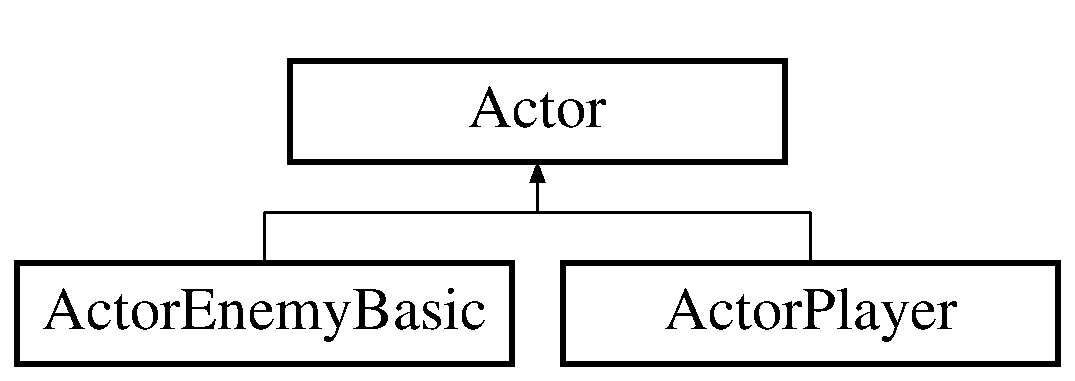
\includegraphics[height=2.000000cm]{class_actor}
\end{center}
\end{figure}
\subsection*{Public Member Functions}
\begin{DoxyCompactItemize}
\item 
\hyperlink{class_actor_a109f99625e52500bf99a94d4f097ad0b}{Actor} (float x\+Posi, float y\+Posi, int hp, int \+\_\+hitbox\+Size, int \hyperlink{class_actor_a87edc76c25d94d8d8c3a09712d554c12}{sprite\+Key})
\begin{DoxyCompactList}\small\item\em Constructor function. \end{DoxyCompactList}\item 
\hyperlink{class_actor_a2a0ff4335a1ee9096df90f288c026c8b}{Actor} ()
\begin{DoxyCompactList}\small\item\em Default constructor function. \end{DoxyCompactList}\item 
virtual \hyperlink{class_actor_ad807fe8f85e72ab263a0c05e3231cb39}{$\sim$\+Actor} ()
\begin{DoxyCompactList}\small\item\em Virtual default destructor function. \end{DoxyCompactList}\item 
float \hyperlink{class_actor_a11aaf02239c93ddb984190de26c42524}{Get\+X\+Coord} ()
\begin{DoxyCompactList}\small\item\em Getter function for x\+Coord. \end{DoxyCompactList}\item 
float \hyperlink{class_actor_a4462d34b9df911fda0b3221819433951}{Get\+Y\+Coord} ()
\begin{DoxyCompactList}\small\item\em Getter function for y\+Coord. \end{DoxyCompactList}\item 
int \hyperlink{class_actor_aabeae30dc510867f0ef39d041f566386}{Get\+Health} ()
\begin{DoxyCompactList}\small\item\em Getter function for health. \end{DoxyCompactList}\item 
int \hyperlink{class_actor_ad36330f5205adfc8a63d79fda3115912}{Get\+Sprite\+Key} ()
\begin{DoxyCompactList}\small\item\em Getter function for sprite\+Key. \end{DoxyCompactList}\item 
void \hyperlink{class_actor_aca64c3d23f52600990f808e5f7ee85eb}{Move\+Actor} ()
\begin{DoxyCompactList}\small\item\em Empty movement function, overloaded by inheriting classes. \end{DoxyCompactList}\item 
void \hyperlink{class_actor_a854aad969c3695d08f335c41f0675ad7}{Set\+X\+Coord} (float new\+Coord)
\begin{DoxyCompactList}\small\item\em Setter function for x\+Coord var. \end{DoxyCompactList}\item 
void \hyperlink{class_actor_aae6e98635555c88a9e19fa1459462f79}{Set\+Y\+Coord} (float new\+Coord)
\begin{DoxyCompactList}\small\item\em Setter function for y\+Coord var. \end{DoxyCompactList}\item 
void \hyperlink{class_actor_a99ae0d6870270e5d9328d7ea4f62c685}{Modify\+Health} (int damage\+Taken)
\begin{DoxyCompactList}\small\item\em Modifies the health variable by a certain amount, mostly used for damaging actors (hence the arg name). \end{DoxyCompactList}\item 
void \hyperlink{class_actor_a7d72c85e4766782f14b7ccf98a1ac503}{Change\+Actor\+Sprite} (int new\+Sprite\+Loc)
\begin{DoxyCompactList}\small\item\em Changes the sprite\+Key index location for the actor\textquotesingle{}s sprite when drawn. \end{DoxyCompactList}\item 
bool \hyperlink{class_actor_af23f6712ddbe46073dfa17918654a21c}{Check\+Dead} ()
\begin{DoxyCompactList}\small\item\em Checks if HP is at/below 0, if so, returns true to allow death resolution logic to occur. Also sets HP to 0 if below. \end{DoxyCompactList}\end{DoxyCompactItemize}
\subsection*{Public Attributes}
\begin{DoxyCompactItemize}
\item 
\hyperlink{class_hitbox}{Hitbox} \hyperlink{class_actor_a3350262199757df220cd955166368ce5}{actor\+Hitbox}
\end{DoxyCompactItemize}
\subsection*{Protected Attributes}
\begin{DoxyCompactItemize}
\item 
float \hyperlink{class_actor_a4877e499ea069ddbab1ba119388e09ae}{x\+Coord}
\item 
float \hyperlink{class_actor_aecada08b60c88c78e2e28b4af48c4baf}{y\+Coord}
\item 
int {\bfseries health}\hypertarget{class_actor_a6932c660e6b6293a66b393c3c9cb151a}{}\label{class_actor_a6932c660e6b6293a66b393c3c9cb151a}

\item 
int {\bfseries hitbox\+Size}\hypertarget{class_actor_a754be3c346e524c21e414e4fec3524e5}{}\label{class_actor_a754be3c346e524c21e414e4fec3524e5}

\item 
int \hyperlink{class_actor_aabe02701e21e0271928ef83c7da7d779}{hitbox\+Width}
\item 
int \hyperlink{class_actor_a87edc76c25d94d8d8c3a09712d554c12}{sprite\+Key}
\end{DoxyCompactItemize}


\subsection{Constructor \& Destructor Documentation}
\index{Actor@{Actor}!Actor@{Actor}}
\index{Actor@{Actor}!Actor@{Actor}}
\subsubsection[{\texorpdfstring{Actor(float x\+Posi, float y\+Posi, int hp, int \+\_\+hitbox\+Size, int sprite\+Key)}{Actor(float xPosi, float yPosi, int hp, int _hitboxSize, int spriteKey)}}]{\setlength{\rightskip}{0pt plus 5cm}Actor\+::\+Actor (
\begin{DoxyParamCaption}
\item[{float}]{x\+Posi, }
\item[{float}]{y\+Posi, }
\item[{int}]{hp, }
\item[{int}]{\+\_\+hitbox\+Size, }
\item[{int}]{sprite\+Key}
\end{DoxyParamCaption}
)}\hypertarget{class_actor_a109f99625e52500bf99a94d4f097ad0b}{}\label{class_actor_a109f99625e52500bf99a94d4f097ad0b}


Constructor function. 

Constructors and Destructors Additional comments about the constructors (if any).

Constructors and Destructors


\begin{DoxyParams}{Parameters}
{\em x\+Posi} & Position on x axis to place new \hyperlink{class_actor}{Actor} at. \\
\hline
{\em y\+Posi} & Position on y axis to place new \hyperlink{class_actor}{Actor} at. \\
\hline
{\em hp} & Health total of the new \hyperlink{class_actor}{Actor}. \\
\hline
{\em \+\_\+hitbox\+Size} & Size of the hitbox that should be constructed as a member. \\
\hline
{\em sprite\+Key} & Location in the sprite index of the actor\textquotesingle{}s sprite bitmap.\\
\hline
\end{DoxyParams}
\begin{DoxyReturn}{Returns}
Initialized \hyperlink{class_actor}{Actor} object. 
\end{DoxyReturn}
\index{Actor@{Actor}!Actor@{Actor}}
\index{Actor@{Actor}!Actor@{Actor}}
\subsubsection[{\texorpdfstring{Actor()}{Actor()}}]{\setlength{\rightskip}{0pt plus 5cm}Actor\+::\+Actor (
\begin{DoxyParamCaption}
{}
\end{DoxyParamCaption}
)}\hypertarget{class_actor_a2a0ff4335a1ee9096df90f288c026c8b}{}\label{class_actor_a2a0ff4335a1ee9096df90f288c026c8b}


Default constructor function. 

\begin{DoxyReturn}{Returns}
Initialized \hyperlink{class_actor}{Actor} object. 
\end{DoxyReturn}
\index{Actor@{Actor}!````~Actor@{$\sim$\+Actor}}
\index{````~Actor@{$\sim$\+Actor}!Actor@{Actor}}
\subsubsection[{\texorpdfstring{$\sim$\+Actor()}{~Actor()}}]{\setlength{\rightskip}{0pt plus 5cm}Actor\+::$\sim$\+Actor (
\begin{DoxyParamCaption}
{}
\end{DoxyParamCaption}
)\hspace{0.3cm}{\ttfamily [virtual]}}\hypertarget{class_actor_ad807fe8f85e72ab263a0c05e3231cb39}{}\label{class_actor_ad807fe8f85e72ab263a0c05e3231cb39}


Virtual default destructor function. 

Additional comments about $\sim$\+Actor virtual destructor (if any).

Declared virtual destructor in order to destruct child classes correctly. 

\subsection{Member Function Documentation}
\index{Actor@{Actor}!Change\+Actor\+Sprite@{Change\+Actor\+Sprite}}
\index{Change\+Actor\+Sprite@{Change\+Actor\+Sprite}!Actor@{Actor}}
\subsubsection[{\texorpdfstring{Change\+Actor\+Sprite(int new\+Sprite\+Loc)}{ChangeActorSprite(int newSpriteLoc)}}]{\setlength{\rightskip}{0pt plus 5cm}Actor\+::\+Change\+Actor\+Sprite (
\begin{DoxyParamCaption}
\item[{int}]{new\+Sprite\+Loc}
\end{DoxyParamCaption}
)}\hypertarget{class_actor_a7d72c85e4766782f14b7ccf98a1ac503}{}\label{class_actor_a7d72c85e4766782f14b7ccf98a1ac503}


Changes the sprite\+Key index location for the actor\textquotesingle{}s sprite when drawn. 

Additional comments about \hyperlink{class_actor_a7d72c85e4766782f14b7ccf98a1ac503}{Change\+Actor\+Sprite()} (if any).


\begin{DoxyParams}{Parameters}
{\em new\+Sprite\+Loc} & The new 3-\/digit index for the sprite\+Index map. \\
\hline
\end{DoxyParams}
\index{Actor@{Actor}!Check\+Dead@{Check\+Dead}}
\index{Check\+Dead@{Check\+Dead}!Actor@{Actor}}
\subsubsection[{\texorpdfstring{Check\+Dead()}{CheckDead()}}]{\setlength{\rightskip}{0pt plus 5cm}Actor\+::\+Check\+Dead (
\begin{DoxyParamCaption}
{}
\end{DoxyParamCaption}
)}\hypertarget{class_actor_af23f6712ddbe46073dfa17918654a21c}{}\label{class_actor_af23f6712ddbe46073dfa17918654a21c}


Checks if HP is at/below 0, if so, returns true to allow death resolution logic to occur. Also sets HP to 0 if below. 

Additional comments about \hyperlink{class_actor_af23f6712ddbe46073dfa17918654a21c}{Check\+Dead()} (if any).

\begin{DoxyReturn}{Returns}
Boolian value. 
\end{DoxyReturn}
\index{Actor@{Actor}!Get\+Health@{Get\+Health}}
\index{Get\+Health@{Get\+Health}!Actor@{Actor}}
\subsubsection[{\texorpdfstring{Get\+Health()}{GetHealth()}}]{\setlength{\rightskip}{0pt plus 5cm}Actor\+::\+Get\+Health (
\begin{DoxyParamCaption}
{}
\end{DoxyParamCaption}
)}\hypertarget{class_actor_aabeae30dc510867f0ef39d041f566386}{}\label{class_actor_aabeae30dc510867f0ef39d041f566386}


Getter function for health. 

Additional comments about \hyperlink{class_actor_aabeae30dc510867f0ef39d041f566386}{Get\+Health()} (if any).

\begin{DoxyReturn}{Returns}
Integer value of health var. 
\end{DoxyReturn}
\index{Actor@{Actor}!Get\+Sprite\+Key@{Get\+Sprite\+Key}}
\index{Get\+Sprite\+Key@{Get\+Sprite\+Key}!Actor@{Actor}}
\subsubsection[{\texorpdfstring{Get\+Sprite\+Key()}{GetSpriteKey()}}]{\setlength{\rightskip}{0pt plus 5cm}Actor\+::\+Get\+Sprite\+Key (
\begin{DoxyParamCaption}
{}
\end{DoxyParamCaption}
)}\hypertarget{class_actor_ad36330f5205adfc8a63d79fda3115912}{}\label{class_actor_ad36330f5205adfc8a63d79fda3115912}


Getter function for sprite\+Key. 

Manipulation Methods

Additional comments about \hyperlink{class_actor_ad36330f5205adfc8a63d79fda3115912}{Get\+Sprite\+Key()} (if any).

\begin{DoxyReturn}{Returns}
Integer value of sprite\+Key var. 
\end{DoxyReturn}
\index{Actor@{Actor}!Get\+X\+Coord@{Get\+X\+Coord}}
\index{Get\+X\+Coord@{Get\+X\+Coord}!Actor@{Actor}}
\subsubsection[{\texorpdfstring{Get\+X\+Coord()}{GetXCoord()}}]{\setlength{\rightskip}{0pt plus 5cm}Actor\+::\+Get\+X\+Coord (
\begin{DoxyParamCaption}
{}
\end{DoxyParamCaption}
)}\hypertarget{class_actor_a11aaf02239c93ddb984190de26c42524}{}\label{class_actor_a11aaf02239c93ddb984190de26c42524}


Getter function for x\+Coord. 

Retrieval methods Additional comments about \hyperlink{class_actor_a11aaf02239c93ddb984190de26c42524}{Get\+X\+Coord()} (if any).

Retrieval Methods

\begin{DoxyReturn}{Returns}
Float value of x\+Coord var. 
\end{DoxyReturn}
\index{Actor@{Actor}!Get\+Y\+Coord@{Get\+Y\+Coord}}
\index{Get\+Y\+Coord@{Get\+Y\+Coord}!Actor@{Actor}}
\subsubsection[{\texorpdfstring{Get\+Y\+Coord()}{GetYCoord()}}]{\setlength{\rightskip}{0pt plus 5cm}Actor\+::\+Get\+Y\+Coord (
\begin{DoxyParamCaption}
{}
\end{DoxyParamCaption}
)}\hypertarget{class_actor_a4462d34b9df911fda0b3221819433951}{}\label{class_actor_a4462d34b9df911fda0b3221819433951}


Getter function for y\+Coord. 

Additional comments about \hyperlink{class_actor_a4462d34b9df911fda0b3221819433951}{Get\+Y\+Coord()} (if any).

\begin{DoxyReturn}{Returns}
Float value of y\+Coord var. 
\end{DoxyReturn}
\index{Actor@{Actor}!Modify\+Health@{Modify\+Health}}
\index{Modify\+Health@{Modify\+Health}!Actor@{Actor}}
\subsubsection[{\texorpdfstring{Modify\+Health(int damage\+Taken)}{ModifyHealth(int damageTaken)}}]{\setlength{\rightskip}{0pt plus 5cm}Actor\+::\+Modify\+Health (
\begin{DoxyParamCaption}
\item[{int}]{damage\+Taken}
\end{DoxyParamCaption}
)}\hypertarget{class_actor_a99ae0d6870270e5d9328d7ea4f62c685}{}\label{class_actor_a99ae0d6870270e5d9328d7ea4f62c685}


Modifies the health variable by a certain amount, mostly used for damaging actors (hence the arg name). 

Manipulation methods Additional comments about \hyperlink{class_actor_a99ae0d6870270e5d9328d7ea4f62c685}{Modify\+Health()} (if any).


\begin{DoxyParams}{Parameters}
{\em damage\+Taken} & The amount to subtract from the \hyperlink{class_actor}{Actor}\textquotesingle{}s health. Will heal the \hyperlink{class_actor}{Actor} if negative. \\
\hline
\end{DoxyParams}
\index{Actor@{Actor}!Move\+Actor@{Move\+Actor}}
\index{Move\+Actor@{Move\+Actor}!Actor@{Actor}}
\subsubsection[{\texorpdfstring{Move\+Actor()}{MoveActor()}}]{\setlength{\rightskip}{0pt plus 5cm}Actor\+::\+Move\+Actor (
\begin{DoxyParamCaption}
{}
\end{DoxyParamCaption}
)}\hypertarget{class_actor_aca64c3d23f52600990f808e5f7ee85eb}{}\label{class_actor_aca64c3d23f52600990f808e5f7ee85eb}


Empty movement function, overloaded by inheriting classes. 

Specific actor types (player, enemies, etc.) should overload this function with that actor type\textquotesingle{}s movement logic. Would have been implemented as a virtual function, however different child classes need different parameters. \index{Actor@{Actor}!Set\+X\+Coord@{Set\+X\+Coord}}
\index{Set\+X\+Coord@{Set\+X\+Coord}!Actor@{Actor}}
\subsubsection[{\texorpdfstring{Set\+X\+Coord(float new\+Coord)}{SetXCoord(float newCoord)}}]{\setlength{\rightskip}{0pt plus 5cm}Actor\+::\+Set\+X\+Coord (
\begin{DoxyParamCaption}
\item[{float}]{new\+Coord}
\end{DoxyParamCaption}
)}\hypertarget{class_actor_a854aad969c3695d08f335c41f0675ad7}{}\label{class_actor_a854aad969c3695d08f335c41f0675ad7}


Setter function for x\+Coord var. 

Additional comments about \hyperlink{class_actor_a854aad969c3695d08f335c41f0675ad7}{Set\+X\+Coord()} (if any).


\begin{DoxyParams}{Parameters}
{\em new\+Coord} & Designates the new horizontal location for the actor object. \\
\hline
\end{DoxyParams}
\index{Actor@{Actor}!Set\+Y\+Coord@{Set\+Y\+Coord}}
\index{Set\+Y\+Coord@{Set\+Y\+Coord}!Actor@{Actor}}
\subsubsection[{\texorpdfstring{Set\+Y\+Coord(float new\+Coord)}{SetYCoord(float newCoord)}}]{\setlength{\rightskip}{0pt plus 5cm}Actor\+::\+Set\+Y\+Coord (
\begin{DoxyParamCaption}
\item[{float}]{new\+Coord}
\end{DoxyParamCaption}
)}\hypertarget{class_actor_aae6e98635555c88a9e19fa1459462f79}{}\label{class_actor_aae6e98635555c88a9e19fa1459462f79}


Setter function for y\+Coord var. 

Additional comments about \hyperlink{class_actor_aae6e98635555c88a9e19fa1459462f79}{Set\+Y\+Coord()} (if any).


\begin{DoxyParams}{Parameters}
{\em new\+Coord} & Designates the new vertical location for the actor object. \\
\hline
\end{DoxyParams}


\subsection{Member Data Documentation}
\index{Actor@{Actor}!actor\+Hitbox@{actor\+Hitbox}}
\index{actor\+Hitbox@{actor\+Hitbox}!Actor@{Actor}}
\subsubsection[{\texorpdfstring{actor\+Hitbox}{actorHitbox}}]{\setlength{\rightskip}{0pt plus 5cm}{\bf Hitbox} Actor\+::actor\+Hitbox}\hypertarget{class_actor_a3350262199757df220cd955166368ce5}{}\label{class_actor_a3350262199757df220cd955166368ce5}
Public member variables Used for collision detection. \index{Actor@{Actor}!hitbox\+Width@{hitbox\+Width}}
\index{hitbox\+Width@{hitbox\+Width}!Actor@{Actor}}
\subsubsection[{\texorpdfstring{hitbox\+Width}{hitboxWidth}}]{\setlength{\rightskip}{0pt plus 5cm}int Actor\+::hitbox\+Width\hspace{0.3cm}{\ttfamily [protected]}}\hypertarget{class_actor_aabe02701e21e0271928ef83c7da7d779}{}\label{class_actor_aabe02701e21e0271928ef83c7da7d779}
health\+: \hyperlink{class_actor}{Actor}\textquotesingle{}s current HP. hitbox\+Size/\+Width\+: Length/width of the member hitbox object. \index{Actor@{Actor}!sprite\+Key@{sprite\+Key}}
\index{sprite\+Key@{sprite\+Key}!Actor@{Actor}}
\subsubsection[{\texorpdfstring{sprite\+Key}{spriteKey}}]{\setlength{\rightskip}{0pt plus 5cm}int Actor\+::sprite\+Key\hspace{0.3cm}{\ttfamily [protected]}}\hypertarget{class_actor_a87edc76c25d94d8d8c3a09712d554c12}{}\label{class_actor_a87edc76c25d94d8d8c3a09712d554c12}
Matches the desired sprite\textquotesingle{}s key within the sprite std\+::map wrapper, used when drawing the actor. \index{Actor@{Actor}!x\+Coord@{x\+Coord}}
\index{x\+Coord@{x\+Coord}!Actor@{Actor}}
\subsubsection[{\texorpdfstring{x\+Coord}{xCoord}}]{\setlength{\rightskip}{0pt plus 5cm}float Actor\+::x\+Coord\hspace{0.3cm}{\ttfamily [protected]}}\hypertarget{class_actor_a4877e499ea069ddbab1ba119388e09ae}{}\label{class_actor_a4877e499ea069ddbab1ba119388e09ae}
Protected member variables \index{Actor@{Actor}!y\+Coord@{y\+Coord}}
\index{y\+Coord@{y\+Coord}!Actor@{Actor}}
\subsubsection[{\texorpdfstring{y\+Coord}{yCoord}}]{\setlength{\rightskip}{0pt plus 5cm}float Actor\+::y\+Coord\hspace{0.3cm}{\ttfamily [protected]}}\hypertarget{class_actor_aecada08b60c88c78e2e28b4af48c4baf}{}\label{class_actor_aecada08b60c88c78e2e28b4af48c4baf}
Determines the location of an actor at a given time. 

The documentation for this class was generated from the following files\+:\begin{DoxyCompactItemize}
\item 
\hyperlink{actor_8h}{actor.\+h}\item 
\hyperlink{actor_8cpp}{actor.\+cpp}\end{DoxyCompactItemize}

\hypertarget{class_actor_enemy_basic}{}\section{Actor\+Enemy\+Basic Class Reference}
\label{class_actor_enemy_basic}\index{Actor\+Enemy\+Basic@{Actor\+Enemy\+Basic}}
Inheritance diagram for Actor\+Enemy\+Basic\+:\begin{figure}[H]
\begin{center}
\leavevmode
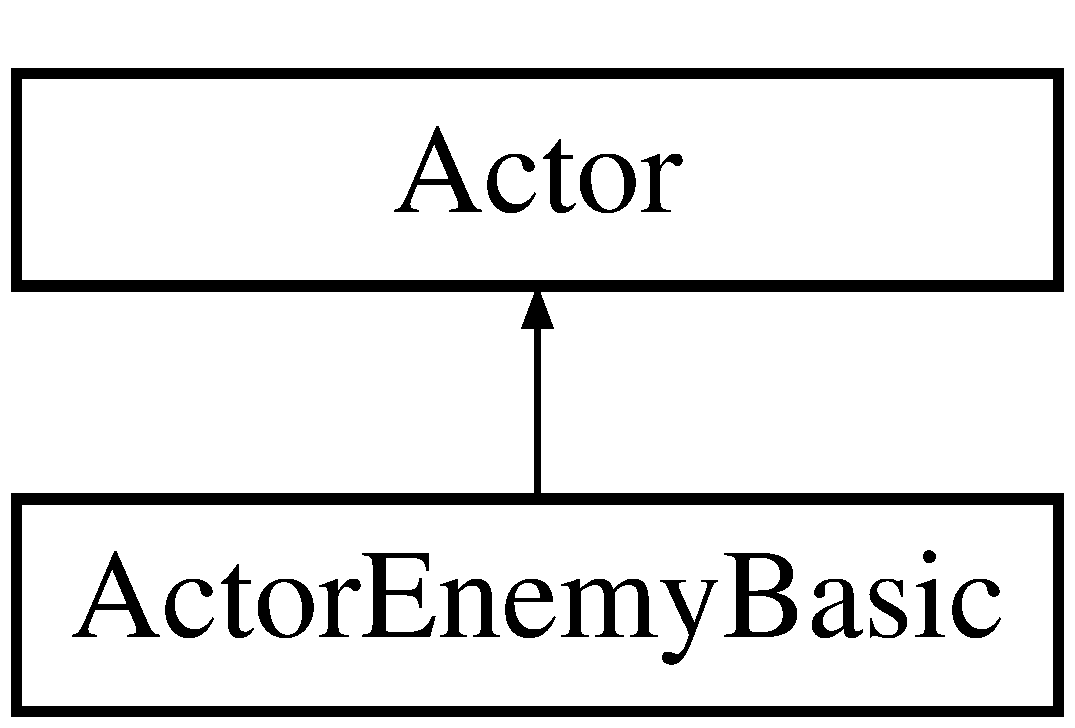
\includegraphics[height=2.000000cm]{class_actor_enemy_basic}
\end{center}
\end{figure}
\subsection*{Public Member Functions}
\begin{DoxyCompactItemize}
\item 
\hyperlink{class_actor_enemy_basic_a316b5d681a568f7cee2880b6cb9bf036}{Actor\+Enemy\+Basic} (float x\+Posi, float y\+Posi, int hp, int \+\_\+hitbox\+Size, int sprite\+Loc, int pts, bool right)
\begin{DoxyCompactList}\small\item\em Constructor function. \end{DoxyCompactList}\item 
void \hyperlink{class_actor_enemy_basic_a63b1ac77626c6c4c78cca1a4e87b17af}{Move\+Actor} (const int M\+O\+V\+E\+R\+A\+T\+E\+\_\+\+A\+C\+T\+O\+RS, const int S\+C\+R\+E\+E\+N\+\_\+\+W\+I\+D\+TH)
\begin{DoxyCompactList}\small\item\em Constructor function. \end{DoxyCompactList}\end{DoxyCompactItemize}
\subsection*{Public Attributes}
\begin{DoxyCompactItemize}
\item 
bool \hyperlink{class_actor_enemy_basic_ad3e644b5068939233cf710b9067868bc}{is\+Dead}
\end{DoxyCompactItemize}
\subsection*{Additional Inherited Members}


\subsection{Constructor \& Destructor Documentation}
\index{Actor\+Enemy\+Basic@{Actor\+Enemy\+Basic}!Actor\+Enemy\+Basic@{Actor\+Enemy\+Basic}}
\index{Actor\+Enemy\+Basic@{Actor\+Enemy\+Basic}!Actor\+Enemy\+Basic@{Actor\+Enemy\+Basic}}
\subsubsection[{\texorpdfstring{Actor\+Enemy\+Basic(float x\+Posi, float y\+Posi, int hp, int \+\_\+hitbox\+Size, int sprite\+Loc, int pts, bool right)}{ActorEnemyBasic(float xPosi, float yPosi, int hp, int _hitboxSize, int spriteLoc, int pts, bool right)}}]{\setlength{\rightskip}{0pt plus 5cm}Actor\+Enemy\+Basic\+::\+Actor\+Enemy\+Basic (
\begin{DoxyParamCaption}
\item[{float}]{x\+Posi, }
\item[{float}]{y\+Posi, }
\item[{int}]{hp, }
\item[{int}]{\+\_\+hitbox\+Size, }
\item[{int}]{sprite\+Loc, }
\item[{int}]{pts, }
\item[{bool}]{right}
\end{DoxyParamCaption}
)}\hypertarget{class_actor_enemy_basic_a316b5d681a568f7cee2880b6cb9bf036}{}\label{class_actor_enemy_basic_a316b5d681a568f7cee2880b6cb9bf036}


Constructor function. 

Constructors and Destructors Additional comments about \hyperlink{class_actor_enemy_basic}{Actor\+Enemy\+Basic} constructors (if any).

Constructors and Destructors


\begin{DoxyParams}{Parameters}
{\em x\+Posi} & Position on x axis to place new \hyperlink{class_actor}{Actor} at. \\
\hline
{\em y\+Posi} & Position on y axis to place new \hyperlink{class_actor}{Actor} at. \\
\hline
{\em hp} & Health total of the new \hyperlink{class_actor}{Actor}. \\
\hline
{\em \+\_\+hitbox\+Size} & Size of the hitbox that should be constructed as a member. \\
\hline
{\em sprite\+Loc} & Location in the sprite index of the actor\textquotesingle{}s sprite bitmap. \\
\hline
{\em pts} & Value of enemy when killed. \\
\hline
{\em right} & Whether the enemy should start moving right(true) or left(false).\\
\hline
\end{DoxyParams}
\begin{DoxyReturn}{Returns}
Initialized \hyperlink{class_actor_enemy_basic}{Actor\+Enemy\+Basic} object. 
\end{DoxyReturn}


\subsection{Member Function Documentation}
\index{Actor\+Enemy\+Basic@{Actor\+Enemy\+Basic}!Move\+Actor@{Move\+Actor}}
\index{Move\+Actor@{Move\+Actor}!Actor\+Enemy\+Basic@{Actor\+Enemy\+Basic}}
\subsubsection[{\texorpdfstring{Move\+Actor(const int M\+O\+V\+E\+R\+A\+T\+E\+\_\+\+A\+C\+T\+O\+R\+S, const int S\+C\+R\+E\+E\+N\+\_\+\+W\+I\+D\+T\+H)}{MoveActor(const int MOVERATE_ACTORS, const int SCREEN_WIDTH)}}]{\setlength{\rightskip}{0pt plus 5cm}Actor\+Enemy\+Basic\+::\+Move\+Actor (
\begin{DoxyParamCaption}
\item[{const int}]{M\+O\+V\+E\+R\+A\+T\+E\+\_\+\+A\+C\+T\+O\+RS, }
\item[{const int}]{S\+C\+R\+E\+E\+N\+\_\+\+W\+I\+D\+TH}
\end{DoxyParamCaption}
)}\hypertarget{class_actor_enemy_basic_a63b1ac77626c6c4c78cca1a4e87b17af}{}\label{class_actor_enemy_basic_a63b1ac77626c6c4c78cca1a4e87b17af}


Constructor function. 

Manipulation Methods Due to the nature of the current movement logic, any enemy unit initialized within x coordinates 0 to 25 and (S\+C\+R\+E\+E\+N\+\_\+\+W\+I\+D\+TH -\/ 25) to S\+C\+R\+E\+E\+N\+\_\+\+W\+I\+D\+TH will simply dive down the screen at a rapid clip. This is a known bug but has not yet been solved. An easy solution is to not spawn basic enemies within those two buffers -\/ be careful when calling the corresponding object\+Spawner function.

Manipulation Methods \begin{DoxyVerb}        Enemy will move right across the gamespace until it comes within
        25 pixels of the edge, at which point it will move its height down
        and reverse movement towards the opposite edge. Loops like this as
        long as the enemy is active.
\end{DoxyVerb}



\begin{DoxyParams}{Parameters}
{\em M\+O\+V\+E\+R\+A\+T\+E\+\_\+\+A\+C\+T\+O\+RS} & Speed at which actors move through the gamespace. \\
\hline
{\em S\+C\+R\+E\+E\+N\+\_\+\+W\+I\+D\+TH} & Width of the screen. \\
\hline
\end{DoxyParams}


\subsection{Member Data Documentation}
\index{Actor\+Enemy\+Basic@{Actor\+Enemy\+Basic}!is\+Dead@{is\+Dead}}
\index{is\+Dead@{is\+Dead}!Actor\+Enemy\+Basic@{Actor\+Enemy\+Basic}}
\subsubsection[{\texorpdfstring{is\+Dead}{isDead}}]{\setlength{\rightskip}{0pt plus 5cm}bool Actor\+Enemy\+Basic\+::is\+Dead}\hypertarget{class_actor_enemy_basic_ad3e644b5068939233cf710b9067868bc}{}\label{class_actor_enemy_basic_ad3e644b5068939233cf710b9067868bc}
Public Member Variables Used to exclude an object from collision while animating its death. 

The documentation for this class was generated from the following files\+:\begin{DoxyCompactItemize}
\item 
\hyperlink{actor_enemy_basic_8h}{actor\+Enemy\+Basic.\+h}\item 
\hyperlink{actor_enemy_basic_8cpp}{actor\+Enemy\+Basic.\+cpp}\end{DoxyCompactItemize}

\hypertarget{class_actor_player}{}\section{Actor\+Player Class Reference}
\label{class_actor_player}\index{Actor\+Player@{Actor\+Player}}
Inheritance diagram for Actor\+Player\+:\begin{figure}[H]
\begin{center}
\leavevmode
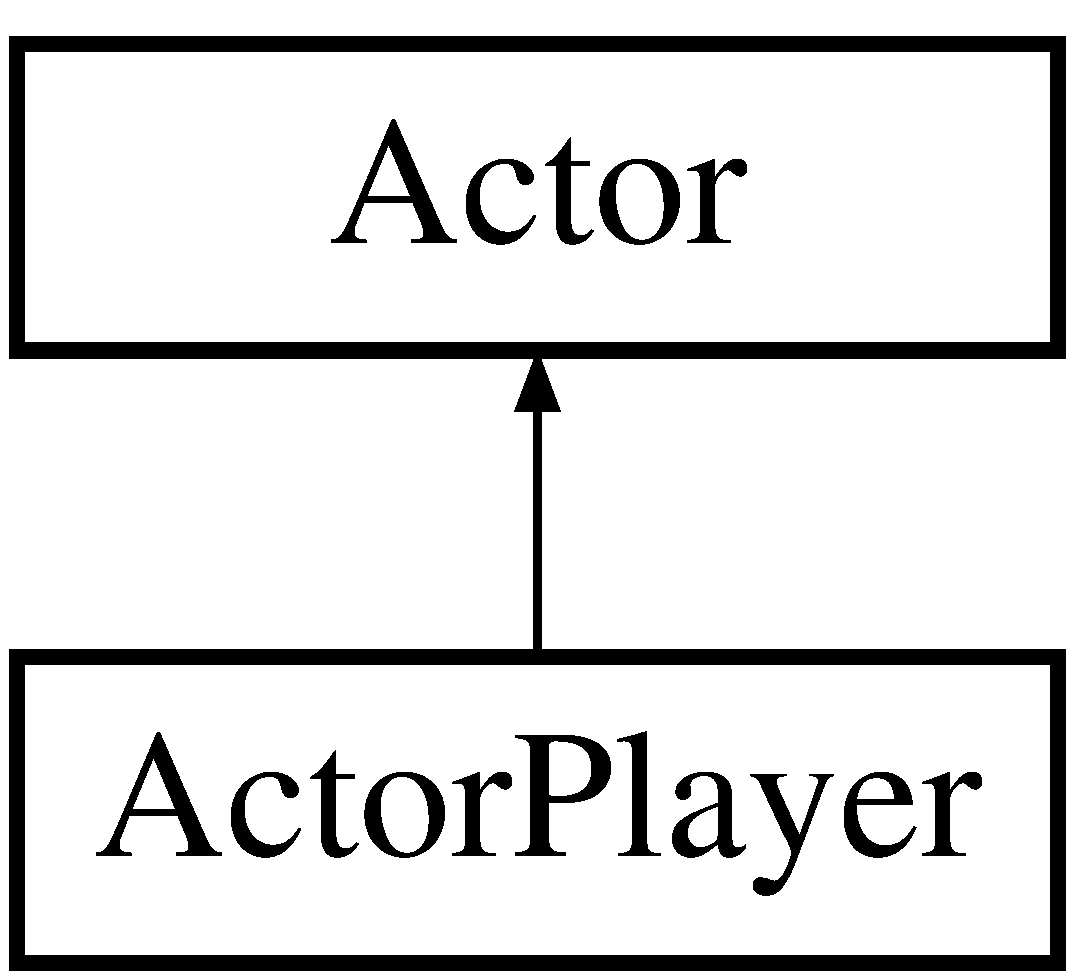
\includegraphics[height=2.000000cm]{class_actor_player}
\end{center}
\end{figure}
\subsection*{Public Member Functions}
\begin{DoxyCompactItemize}
\item 
\hyperlink{class_actor_player_aa12290932cca3cda19f8d6211923d273}{Actor\+Player} (float x\+Posi, float y\+Posi, int hp, int \+\_\+hitbox\+Size, int sprite\+Loc)
\begin{DoxyCompactList}\small\item\em Constructor function. \end{DoxyCompactList}\item 
int \hyperlink{class_actor_player_ad8e2322c07d45cfafac93535fc6426ee}{Get\+Score} ()
\begin{DoxyCompactList}\small\item\em Returns current player score amount. \end{DoxyCompactList}\item 
int \hyperlink{class_actor_player_a69cac19946ff088df3b06f33ac32377b}{Get\+Lives} ()
\begin{DoxyCompactList}\small\item\em Returns current player life total. \end{DoxyCompactList}\item 
void \hyperlink{class_actor_player_a97a34c50516109aaf4743a9880604145}{Move\+Actor} (bool move\+Up, bool move\+Down, bool move\+Left, bool move\+Right, const int M\+O\+V\+E\+R\+A\+T\+E\+\_\+\+A\+C\+T\+O\+RS)
\begin{DoxyCompactList}\small\item\em When passed a series of bools, moves the actor appropriately. \end{DoxyCompactList}\item 
void \hyperlink{class_actor_player_a2a7f5b152ea4bb8d283281e8bad1bdf0}{Update\+Score} (int score\+Gained)
\begin{DoxyCompactList}\small\item\em Updates the player\textquotesingle{}s score by a specified amount. \end{DoxyCompactList}\item 
void \hyperlink{class_actor_player_aea4f9b0c8caa624b5cd48d88e7634aab}{Set\+Lives} (int new\+Life\+Total)
\begin{DoxyCompactList}\small\item\em Sets the player\textquotesingle{}s life total to a new value. \end{DoxyCompactList}\item 
void \hyperlink{class_actor_player_ad93f5fd94f72b720763c561f3f729a8b}{Kill\+Player} (int new\+Sprite\+Loc, float default\+X\+Posi, float default\+Y\+Posi)
\begin{DoxyCompactList}\small\item\em Decrements lives by 1, changes the player sprite\+Index key, and moves the player back to the starting position. \end{DoxyCompactList}\end{DoxyCompactItemize}
\subsection*{Public Attributes}
\begin{DoxyCompactItemize}
\item 
int \hyperlink{class_actor_player_a9f866cfd729bcaee1138fdfab5010422}{bullet\+Control\+Counter}
\end{DoxyCompactItemize}
\subsection*{Additional Inherited Members}


\subsection{Constructor \& Destructor Documentation}
\index{Actor\+Player@{Actor\+Player}!Actor\+Player@{Actor\+Player}}
\index{Actor\+Player@{Actor\+Player}!Actor\+Player@{Actor\+Player}}
\subsubsection[{\texorpdfstring{Actor\+Player(float x\+Posi, float y\+Posi, int hp, int \+\_\+hitbox\+Size, int sprite\+Loc)}{ActorPlayer(float xPosi, float yPosi, int hp, int _hitboxSize, int spriteLoc)}}]{\setlength{\rightskip}{0pt plus 5cm}Actor\+Player\+::\+Actor\+Player (
\begin{DoxyParamCaption}
\item[{float}]{x\+Posi, }
\item[{float}]{y\+Posi, }
\item[{int}]{hp, }
\item[{int}]{\+\_\+hitbox\+Size, }
\item[{int}]{sprite\+Key}
\end{DoxyParamCaption}
)}\hypertarget{class_actor_player_aa12290932cca3cda19f8d6211923d273}{}\label{class_actor_player_aa12290932cca3cda19f8d6211923d273}


Constructor function. 

Constructors and Destructors player\+Score is initialized to 0 for obvious reasons. The constructor should be expanded however to allow initialization of lives. bullet\+Control\+Counter is set to 5 by default, as this is the value checked for in main when allowing the player to fire. Ergo, a newly constructed \hyperlink{class_actor_player}{Actor\+Player} object can fire on its first update cycle if the player chooses.

Constructors and Destructors


\begin{DoxyParams}{Parameters}
{\em x\+Posi} & Position on x axis to place new \hyperlink{class_actor_player}{Actor\+Player} at. \\
\hline
{\em y\+Posi} & Position on y axis to place new \hyperlink{class_actor_player}{Actor\+Player} at. \\
\hline
{\em hp} & Health total of the new \hyperlink{class_actor_player}{Actor\+Player}. \\
\hline
{\em \+\_\+hitbox\+Size} & Size of the hitbox that should be constructed as a member. \\
\hline
{\em sprite\+Loc} & Location in the sprite index of the \hyperlink{class_actor_player}{Actor\+Player} sprite bitmap.\\
\hline
\end{DoxyParams}
\begin{DoxyReturn}{Returns}
Initialized \hyperlink{class_actor_player}{Actor\+Player} object. 
\end{DoxyReturn}


\subsection{Member Function Documentation}
\index{Actor\+Player@{Actor\+Player}!Get\+Lives@{Get\+Lives}}
\index{Get\+Lives@{Get\+Lives}!Actor\+Player@{Actor\+Player}}
\subsubsection[{\texorpdfstring{Get\+Lives()}{GetLives()}}]{\setlength{\rightskip}{0pt plus 5cm}Actor\+Player\+::\+Get\+Lives (
\begin{DoxyParamCaption}
{}
\end{DoxyParamCaption}
)}\hypertarget{class_actor_player_a69cac19946ff088df3b06f33ac32377b}{}\label{class_actor_player_a69cac19946ff088df3b06f33ac32377b}


Returns current player life total. 

Additional comments about Get\+Lives method (if any).

\begin{DoxyReturn}{Returns}
Integer value. 
\end{DoxyReturn}
\index{Actor\+Player@{Actor\+Player}!Get\+Score@{Get\+Score}}
\index{Get\+Score@{Get\+Score}!Actor\+Player@{Actor\+Player}}
\subsubsection[{\texorpdfstring{Get\+Score()}{GetScore()}}]{\setlength{\rightskip}{0pt plus 5cm}Actor\+Player\+::\+Get\+Score (
\begin{DoxyParamCaption}
{}
\end{DoxyParamCaption}
)}\hypertarget{class_actor_player_ad8e2322c07d45cfafac93535fc6426ee}{}\label{class_actor_player_ad8e2322c07d45cfafac93535fc6426ee}


Returns current player score amount. 

Additional comments about Get\+Score method (if any).

Retrieval Methods

\begin{DoxyReturn}{Returns}
Integer value. 
\end{DoxyReturn}
\index{Actor\+Player@{Actor\+Player}!Kill\+Player@{Kill\+Player}}
\index{Kill\+Player@{Kill\+Player}!Actor\+Player@{Actor\+Player}}
\subsubsection[{\texorpdfstring{Kill\+Player(int new\+Sprite\+Loc, float default\+X\+Posi, float default\+Y\+Posi)}{KillPlayer(int newSpriteLoc, float defaultXPosi, float defaultYPosi)}}]{\setlength{\rightskip}{0pt plus 5cm}Actor\+Player\+::\+Kill\+Player (
\begin{DoxyParamCaption}
\item[{int}]{new\+Sprite\+Loc, }
\item[{float}]{default\+X\+Posi, }
\item[{float}]{default\+Y\+Posi}
\end{DoxyParamCaption}
)}\hypertarget{class_actor_player_ad93f5fd94f72b720763c561f3f729a8b}{}\label{class_actor_player_ad93f5fd94f72b720763c561f3f729a8b}


Decrements lives by 1, changes the player sprite\+Index key, and moves the player back to the starting position. 

This entire function should be rewritten and can probably be replaced wholesale by a series of getter/setter functions and existing code calls external to the class. It probably doesn\textquotesingle{}t need to be here, but it serves its purpose in the code as it stands.


\begin{DoxyParams}{Parameters}
{\em new\+Sprite\+Loc} & The key to the player\textquotesingle{}s new sprite (can be the same as the current sprite if desired). \\
\hline
{\em default\+X\+Posi} & The location on the x axis to place the player (should usually be the same as the place the player starts initially). \\
\hline
{\em default\+Y\+Posi} & The location on the y axis to place the player (should usually be the same as the place the player starts initially). \begin{DoxyVerb}        This code needs to be rewritten, not for functionality (it works fine) but because it's ugly and stylistically undesirable. However,
        time constraints mean it won't be.\end{DoxyVerb}
 \\
\hline
\end{DoxyParams}
\index{Actor\+Player@{Actor\+Player}!Move\+Actor@{Move\+Actor}}
\index{Move\+Actor@{Move\+Actor}!Actor\+Player@{Actor\+Player}}
\subsubsection[{\texorpdfstring{Move\+Actor(bool move\+Up, bool move\+Down, bool move\+Left, bool move\+Right, const int M\+O\+V\+E\+R\+A\+T\+E\+\_\+\+A\+C\+T\+O\+R\+S)}{MoveActor(bool moveUp, bool moveDown, bool moveLeft, bool moveRight, const int MOVERATE_ACTORS)}}]{\setlength{\rightskip}{0pt plus 5cm}Actor\+Player\+::\+Move\+Actor (
\begin{DoxyParamCaption}
\item[{bool}]{move\+Up, }
\item[{bool}]{move\+Down, }
\item[{bool}]{move\+Left, }
\item[{bool}]{move\+Right, }
\item[{const int}]{M\+O\+V\+E\+R\+A\+T\+E\+\_\+\+A\+C\+T\+O\+RS}
\end{DoxyParamCaption}
)}\hypertarget{class_actor_player_a97a34c50516109aaf4743a9880604145}{}\label{class_actor_player_a97a34c50516109aaf4743a9880604145}


When passed a series of bools, moves the actor appropriately. 

The magic numbers used here correspond to the screen edges necessary to make the player stop 10 pixels from the screen edge. A file should really be defined to allow access to those variable values for this purpose, as it would avoid needing to pass four+ const int vars to each function that needs to know (which keeps the arguments much tidier).

Manipulation Methods


\begin{DoxyParams}{Parameters}
{\em move\+Up} & If true, the actor will move upwards a distance defined by the moverate. \\
\hline
{\em move\+Down} & If true, the actor will move downwards a distance defined by the moverate. \\
\hline
{\em move\+Left} & If true, the actor will move left a distance defined by the moverate. \\
\hline
{\em move\+Right} & If true, the actor will move right a distance defined by the moverate. \\
\hline
{\em M\+O\+V\+E\+R\+A\+T\+E\+\_\+\+A\+C\+T\+O\+RS} & The number of pixels to move the actor\textquotesingle{}s location in a given direction. \begin{DoxyVerb}        This function is intended to be fed information based on keypress values. For an example
        implementation, see the main function.\end{DoxyVerb}
 \\
\hline
\end{DoxyParams}
\index{Actor\+Player@{Actor\+Player}!Set\+Lives@{Set\+Lives}}
\index{Set\+Lives@{Set\+Lives}!Actor\+Player@{Actor\+Player}}
\subsubsection[{\texorpdfstring{Set\+Lives(int new\+Life\+Total)}{SetLives(int newLifeTotal)}}]{\setlength{\rightskip}{0pt plus 5cm}Actor\+Player\+::\+Set\+Lives (
\begin{DoxyParamCaption}
\item[{int}]{new\+Life\+Total}
\end{DoxyParamCaption}
)}\hypertarget{class_actor_player_aea4f9b0c8caa624b5cd48d88e7634aab}{}\label{class_actor_player_aea4f9b0c8caa624b5cd48d88e7634aab}


Sets the player\textquotesingle{}s life total to a new value. 

Additional comments about Set\+Lives method (if any).


\begin{DoxyParams}{Parameters}
{\em new\+Life\+Total} & The new value to assign to lives member. \\
\hline
\end{DoxyParams}
\index{Actor\+Player@{Actor\+Player}!Update\+Score@{Update\+Score}}
\index{Update\+Score@{Update\+Score}!Actor\+Player@{Actor\+Player}}
\subsubsection[{\texorpdfstring{Update\+Score(int score\+Gained)}{UpdateScore(int scoreGained)}}]{\setlength{\rightskip}{0pt plus 5cm}Actor\+Player\+::\+Update\+Score (
\begin{DoxyParamCaption}
\item[{int}]{score\+Gained}
\end{DoxyParamCaption}
)}\hypertarget{class_actor_player_a2a7f5b152ea4bb8d283281e8bad1bdf0}{}\label{class_actor_player_a2a7f5b152ea4bb8d283281e8bad1bdf0}


Updates the player\textquotesingle{}s score by a specified amount. 

Additional comments about Update\+Score method (if any).


\begin{DoxyParams}{Parameters}
{\em score\+Gained} & Increases player\+Score by the specified amount. If negative, will decrease player\+Score instead. \begin{DoxyVerb}        This function is not currently used.\end{DoxyVerb}
 \\
\hline
\end{DoxyParams}


\subsection{Member Data Documentation}
\index{Actor\+Player@{Actor\+Player}!bullet\+Control\+Counter@{bullet\+Control\+Counter}}
\index{bullet\+Control\+Counter@{bullet\+Control\+Counter}!Actor\+Player@{Actor\+Player}}
\subsubsection[{\texorpdfstring{bullet\+Control\+Counter}{bulletControlCounter}}]{\setlength{\rightskip}{0pt plus 5cm}int Actor\+Player\+::bullet\+Control\+Counter}\hypertarget{class_actor_player_a9f866cfd729bcaee1138fdfab5010422}{}\label{class_actor_player_a9f866cfd729bcaee1138fdfab5010422}
Public Member Variables Used to count update cycles, such that a player must wait at least x update cycles before firing a second projectile. 

The documentation for this class was generated from the following files\+:\begin{DoxyCompactItemize}
\item 
\hyperlink{actor_player_8h}{actor\+Player.\+h}\item 
\hyperlink{actor_player_8cpp}{actor\+Player.\+cpp}\end{DoxyCompactItemize}

\hypertarget{class_hitbox}{}\section{Hitbox Class Reference}
\label{class_hitbox}\index{Hitbox@{Hitbox}}
\subsection*{Public Member Functions}
\begin{DoxyCompactItemize}
\item 
\hyperlink{class_hitbox_acb9da54b168b9e457b01387ba4ddfe02}{Hitbox} (float x, float y, int width, int length)
\begin{DoxyCompactList}\small\item\em Constructor function. \end{DoxyCompactList}\item 
\hyperlink{class_hitbox_a999b0be8486978b3dd7bcd001c7c3c03}{Hitbox} ()
\begin{DoxyCompactList}\small\item\em Default constructor function. \end{DoxyCompactList}\item 
float \hyperlink{class_hitbox_afa9e21136ddd399793bbd375af5f16cc}{Get\+HitboxX} ()
\begin{DoxyCompactList}\small\item\em Returns current \hyperlink{class_hitbox}{Hitbox} centred x coordinate. \end{DoxyCompactList}\item 
float \hyperlink{class_hitbox_af1fbffe46fd19d47019514744144fa1d}{Get\+HitboxY} ()
\begin{DoxyCompactList}\small\item\em Returns current \hyperlink{class_hitbox}{Hitbox} centred y coordinate. \end{DoxyCompactList}\item 
float \hyperlink{class_hitbox_a318a7a3694024fa394b8d35ecd36ccdd}{Get\+Hitbox\+Width} ()
\begin{DoxyCompactList}\small\item\em Returns width of \hyperlink{class_hitbox}{Hitbox} (measured as pixels on either side of central pixel). \end{DoxyCompactList}\item 
float \hyperlink{class_hitbox_ac500587c4afac7159161affbbd46f3b3}{Get\+Hitbox\+Height} ()
\begin{DoxyCompactList}\small\item\em Returns height of \hyperlink{class_hitbox}{Hitbox} (measured as pixels on either side of central pixel). \end{DoxyCompactList}\item 
void \hyperlink{class_hitbox_a6f4500fa0f6c8dd9aeb9ab74c24fa6b8}{Move\+Hitbox} (float new\+X\+Location, float new\+Y\+Location)
\begin{DoxyCompactList}\small\item\em Moves the centre of the hitbox to a new location. \end{DoxyCompactList}\item 
bool \hyperlink{class_hitbox_a02f19a92f5cf1bd5ff917e9e9a875b37}{Check\+For\+Collision} (\hyperlink{class_hitbox}{Hitbox} target)
\begin{DoxyCompactList}\small\item\em Checks if the current \hyperlink{class_hitbox}{Hitbox} is inside another \hyperlink{class_hitbox}{Hitbox} at any location. \end{DoxyCompactList}\end{DoxyCompactItemize}


\subsection{Constructor \& Destructor Documentation}
\index{Hitbox@{Hitbox}!Hitbox@{Hitbox}}
\index{Hitbox@{Hitbox}!Hitbox@{Hitbox}}
\subsubsection[{\texorpdfstring{Hitbox(float x, float y, int width, int length)}{Hitbox(float x, float y, int width, int length)}}]{\setlength{\rightskip}{0pt plus 5cm}Hitbox\+::\+Hitbox (
\begin{DoxyParamCaption}
\item[{float}]{x, }
\item[{float}]{y, }
\item[{int}]{width, }
\item[{int}]{length}
\end{DoxyParamCaption}
)}\hypertarget{class_hitbox_acb9da54b168b9e457b01387ba4ddfe02}{}\label{class_hitbox_acb9da54b168b9e457b01387ba4ddfe02}


Constructor function. 

Constructors and Destructors Additional comments about \hyperlink{class_hitbox}{Hitbox} constructors (if any).

Constructors and Destructors


\begin{DoxyParams}{Parameters}
{\em x} & Position on x axis to centre new \hyperlink{class_hitbox}{Hitbox} at. \\
\hline
{\em y} & Position on y axis to centre new \hyperlink{class_hitbox}{Hitbox} at. \\
\hline
{\em width} & Width of hitbox (measured as number of pixels on either side of the central pixel). \\
\hline
{\em length} & Length of hitbox (measured as number of pixels on either side of the central pixel).\\
\hline
\end{DoxyParams}
\begin{DoxyReturn}{Returns}
Initialized \hyperlink{class_hitbox}{Hitbox} object. 
\end{DoxyReturn}
\index{Hitbox@{Hitbox}!Hitbox@{Hitbox}}
\index{Hitbox@{Hitbox}!Hitbox@{Hitbox}}
\subsubsection[{\texorpdfstring{Hitbox()}{Hitbox()}}]{\setlength{\rightskip}{0pt plus 5cm}Hitbox\+::\+Hitbox (
\begin{DoxyParamCaption}
{}
\end{DoxyParamCaption}
)}\hypertarget{class_hitbox_a999b0be8486978b3dd7bcd001c7c3c03}{}\label{class_hitbox_a999b0be8486978b3dd7bcd001c7c3c03}


Default constructor function. 

\begin{DoxyReturn}{Returns}
Initialized \hyperlink{class_hitbox}{Hitbox} object. 
\end{DoxyReturn}


\subsection{Member Function Documentation}
\index{Hitbox@{Hitbox}!Check\+For\+Collision@{Check\+For\+Collision}}
\index{Check\+For\+Collision@{Check\+For\+Collision}!Hitbox@{Hitbox}}
\subsubsection[{\texorpdfstring{Check\+For\+Collision(\+Hitbox target)}{CheckForCollision(Hitbox target)}}]{\setlength{\rightskip}{0pt plus 5cm}Hitbox\+::\+Check\+For\+Collision (
\begin{DoxyParamCaption}
\item[{{\bf Hitbox}}]{target}
\end{DoxyParamCaption}
)}\hypertarget{class_hitbox_a02f19a92f5cf1bd5ff917e9e9a875b37}{}\label{class_hitbox_a02f19a92f5cf1bd5ff917e9e9a875b37}


Checks if the current \hyperlink{class_hitbox}{Hitbox} is inside another \hyperlink{class_hitbox}{Hitbox} at any location. 

Additional comments about Check\+For\+Collision method (if any).


\begin{DoxyParams}{Parameters}
{\em target} & \hyperlink{class_hitbox}{Hitbox} object to determine collision with. \begin{DoxyVerb}        True is returned if the current and target hitboxes are intersecting at any point, at this moment.
        Does not check along paths. If objects move in large enough spans per update cycle, an algorithm
        may be needed to prevent objects "skipping" over each other. 
\end{DoxyVerb}
\\
\hline
\end{DoxyParams}
\begin{DoxyReturn}{Returns}
Boolian value. 
\end{DoxyReturn}
\index{Hitbox@{Hitbox}!Get\+Hitbox\+Height@{Get\+Hitbox\+Height}}
\index{Get\+Hitbox\+Height@{Get\+Hitbox\+Height}!Hitbox@{Hitbox}}
\subsubsection[{\texorpdfstring{Get\+Hitbox\+Height()}{GetHitboxHeight()}}]{\setlength{\rightskip}{0pt plus 5cm}Hitbox\+::\+Get\+Hitbox\+Height (
\begin{DoxyParamCaption}
{}
\end{DoxyParamCaption}
)}\hypertarget{class_hitbox_ac500587c4afac7159161affbbd46f3b3}{}\label{class_hitbox_ac500587c4afac7159161affbbd46f3b3}


Returns height of \hyperlink{class_hitbox}{Hitbox} (measured as pixels on either side of central pixel). 

Additional comments about Get\+Hitbox\+Height method (if any).

\begin{DoxyReturn}{Returns}
Float value. 
\end{DoxyReturn}
\index{Hitbox@{Hitbox}!Get\+Hitbox\+Width@{Get\+Hitbox\+Width}}
\index{Get\+Hitbox\+Width@{Get\+Hitbox\+Width}!Hitbox@{Hitbox}}
\subsubsection[{\texorpdfstring{Get\+Hitbox\+Width()}{GetHitboxWidth()}}]{\setlength{\rightskip}{0pt plus 5cm}Hitbox\+::\+Get\+Hitbox\+Width (
\begin{DoxyParamCaption}
{}
\end{DoxyParamCaption}
)}\hypertarget{class_hitbox_a318a7a3694024fa394b8d35ecd36ccdd}{}\label{class_hitbox_a318a7a3694024fa394b8d35ecd36ccdd}


Returns width of \hyperlink{class_hitbox}{Hitbox} (measured as pixels on either side of central pixel). 

Additional comments about Get\+Hitbox\+Width method (if any).

\begin{DoxyReturn}{Returns}
Float value. 
\end{DoxyReturn}
\index{Hitbox@{Hitbox}!Get\+HitboxX@{Get\+HitboxX}}
\index{Get\+HitboxX@{Get\+HitboxX}!Hitbox@{Hitbox}}
\subsubsection[{\texorpdfstring{Get\+Hitbox\+X()}{GetHitboxX()}}]{\setlength{\rightskip}{0pt plus 5cm}Hitbox\+::\+Get\+HitboxX (
\begin{DoxyParamCaption}
{}
\end{DoxyParamCaption}
)}\hypertarget{class_hitbox_afa9e21136ddd399793bbd375af5f16cc}{}\label{class_hitbox_afa9e21136ddd399793bbd375af5f16cc}


Returns current \hyperlink{class_hitbox}{Hitbox} centred x coordinate. 

Retrieval Methods Additional comments about Get\+HitboxX method (if any).

Retrieval Methods

\begin{DoxyReturn}{Returns}
Float value. 
\end{DoxyReturn}
\index{Hitbox@{Hitbox}!Get\+HitboxY@{Get\+HitboxY}}
\index{Get\+HitboxY@{Get\+HitboxY}!Hitbox@{Hitbox}}
\subsubsection[{\texorpdfstring{Get\+Hitbox\+Y()}{GetHitboxY()}}]{\setlength{\rightskip}{0pt plus 5cm}Hitbox\+::\+Get\+HitboxY (
\begin{DoxyParamCaption}
{}
\end{DoxyParamCaption}
)}\hypertarget{class_hitbox_af1fbffe46fd19d47019514744144fa1d}{}\label{class_hitbox_af1fbffe46fd19d47019514744144fa1d}


Returns current \hyperlink{class_hitbox}{Hitbox} centred y coordinate. 

Additional comments about Get\+HitboxY method (if any).

\begin{DoxyReturn}{Returns}
Float value. 
\end{DoxyReturn}
\index{Hitbox@{Hitbox}!Move\+Hitbox@{Move\+Hitbox}}
\index{Move\+Hitbox@{Move\+Hitbox}!Hitbox@{Hitbox}}
\subsubsection[{\texorpdfstring{Move\+Hitbox(float new\+X\+Location, float new\+Y\+Location)}{MoveHitbox(float newXLocation, float newYLocation)}}]{\setlength{\rightskip}{0pt plus 5cm}Hitbox\+::\+Move\+Hitbox (
\begin{DoxyParamCaption}
\item[{float}]{new\+X\+Location, }
\item[{float}]{new\+Y\+Location}
\end{DoxyParamCaption}
)}\hypertarget{class_hitbox_a6f4500fa0f6c8dd9aeb9ab74c24fa6b8}{}\label{class_hitbox_a6f4500fa0f6c8dd9aeb9ab74c24fa6b8}


Moves the centre of the hitbox to a new location. 

Manipulation Methods Additional comments about Move\+Hitbox method (if any).

Manipulation Methods


\begin{DoxyParams}{Parameters}
{\em new\+X\+Location} & New horizontal location for central pixel of hitbox. \\
\hline
{\em new\+Y\+Location} & New vertical location for central pixel of hitbox. \\
\hline
\end{DoxyParams}


The documentation for this class was generated from the following files\+:\begin{DoxyCompactItemize}
\item 
\hyperlink{_hitbox_8h}{Hitbox.\+h}\item 
\hyperlink{_hitbox_8cpp}{Hitbox.\+cpp}\end{DoxyCompactItemize}

\hypertarget{class_projectile}{}\section{Projectile Class Reference}
\label{class_projectile}\index{Projectile@{Projectile}}
Inheritance diagram for Projectile\+:\begin{figure}[H]
\begin{center}
\leavevmode
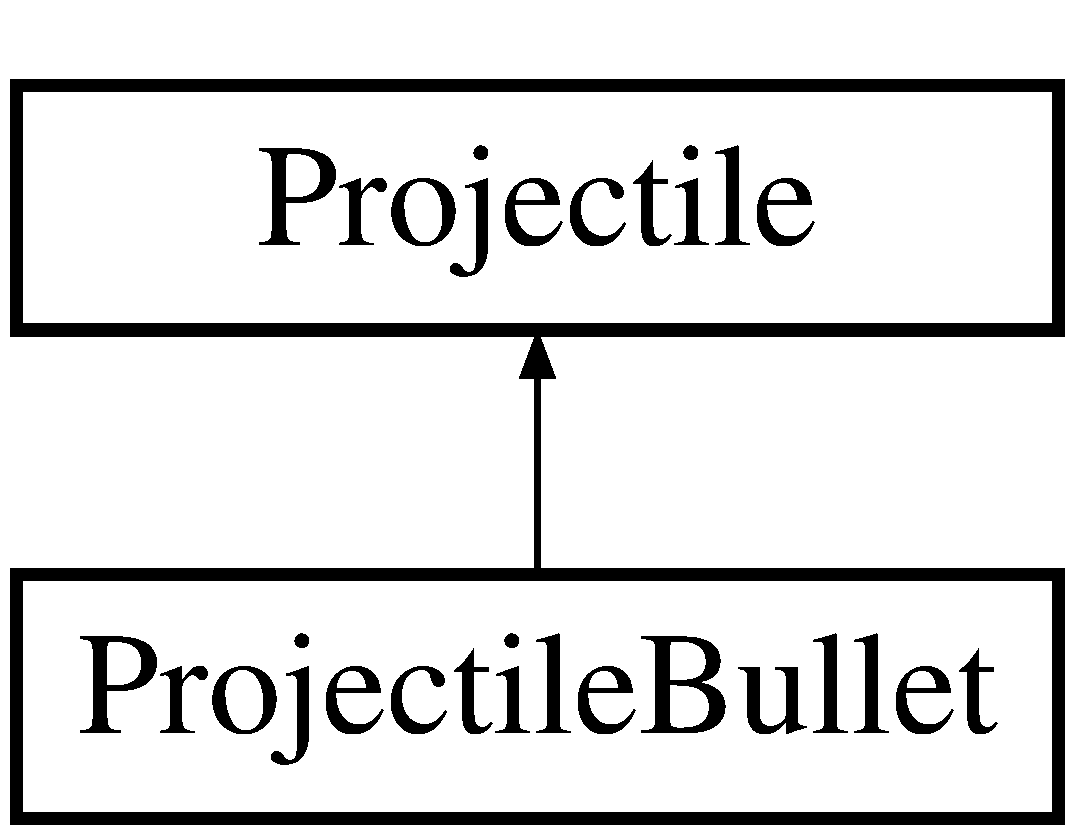
\includegraphics[height=2.000000cm]{class_projectile}
\end{center}
\end{figure}
\subsection*{Public Member Functions}
\begin{DoxyCompactItemize}
\item 
\hyperlink{class_projectile_a9f5c35e63c72e01ecc6a2b9d0b250aff}{Projectile} (float x\+Posi, float y\+Posi, int dir, int \+\_\+hitbox\+Size)
\begin{DoxyCompactList}\small\item\em Constructor function. \end{DoxyCompactList}\item 
virtual \hyperlink{class_projectile_a94903e021fa2edab60ba3836ca0b937d}{$\sim$\+Projectile} ()
\begin{DoxyCompactList}\small\item\em Virtual default constructor function. \end{DoxyCompactList}\item 
float \hyperlink{class_projectile_aefcef09fde3c66ddbbcc58f599bd7965}{Get\+X\+Coord} ()
\begin{DoxyCompactList}\small\item\em Exposes and returns x\+Coordinate. \end{DoxyCompactList}\item 
float \hyperlink{class_projectile_a2c5fabef6aa3fc8831717a2b1751adcd}{Get\+Y\+Coord} ()
\begin{DoxyCompactList}\small\item\em Exposes and returns y\+Coordinate. \end{DoxyCompactList}\item 
void \hyperlink{class_projectile_a9eff3315fef4f92927d52dd9372a3f35}{Move\+Projectile} (const int M\+O\+V\+E\+R\+A\+T\+E\+\_\+\+P\+R\+O\+J\+E\+C\+T\+I\+L\+ES)
\begin{DoxyCompactList}\small\item\em Moves the single-\/pixel location of a projectile a given distance down or up. Modifies x\+Coordinate and y\+Coordinate. \end{DoxyCompactList}\item 
void \hyperlink{class_projectile_a47422fcf423ec9068329fe899a571e62}{Draw\+Projectile} ()
\end{DoxyCompactItemize}
\subsection*{Public Attributes}
\begin{DoxyCompactItemize}
\item 
\hyperlink{class_hitbox}{Hitbox} \hyperlink{class_projectile_ae0036dcb811aabf0228f768700491790}{projectile\+Hitbox}
\item 
bool \hyperlink{class_projectile_aae745fd2564addc23d5456fe5fd1a711}{proj\+Inactive}
\end{DoxyCompactItemize}
\subsection*{Protected Types}
\begin{DoxyCompactItemize}
\item 
enum {\bfseries directions\+\_\+c} \{ {\bfseries UP}, 
{\bfseries D\+O\+WN}
 \}\hypertarget{class_projectile_ad4b7defda550e55015b594db2d85644c}{}\label{class_projectile_ad4b7defda550e55015b594db2d85644c}

\end{DoxyCompactItemize}
\subsection*{Protected Attributes}
\begin{DoxyCompactItemize}
\item 
float \hyperlink{class_projectile_a744bb0d2fd11da1750ab875ceea4b5cb}{x\+Coordinate}
\item 
float \hyperlink{class_projectile_a23383eb9240ee101dbdacbcc87b0a920}{y\+Coordinate}
\item 
directions\+\_\+c \hyperlink{class_projectile_a31cb4995dad27c6b37dd8a312edbd5af}{bullet\+Direction}
\end{DoxyCompactItemize}


\subsection{Constructor \& Destructor Documentation}
\index{Projectile@{Projectile}!Projectile@{Projectile}}
\index{Projectile@{Projectile}!Projectile@{Projectile}}
\subsubsection[{\texorpdfstring{Projectile(float x\+Posi, float y\+Posi, int dir, int \+\_\+hitbox\+Size)}{Projectile(float xPosi, float yPosi, int dir, int _hitboxSize)}}]{\setlength{\rightskip}{0pt plus 5cm}Projectile\+::\+Projectile (
\begin{DoxyParamCaption}
\item[{float}]{x\+Posi, }
\item[{float}]{y\+Posi, }
\item[{int}]{dir, }
\item[{int}]{\+\_\+hitbox\+Size}
\end{DoxyParamCaption}
)}\hypertarget{class_projectile_a9f5c35e63c72e01ecc6a2b9d0b250aff}{}\label{class_projectile_a9f5c35e63c72e01ecc6a2b9d0b250aff}


Constructor function. 

Private Methods Public Methods bullet\+Direction is taken as as an int in the constructor because directions\+\_\+c is an enum only declared in the class.

Constructors and Destructors


\begin{DoxyParams}{Parameters}
{\em x\+Posi} & Position on x axis to place new \hyperlink{class_projectile}{Projectile} at. \\
\hline
{\em y\+Posi} & Position on y axis to place new \hyperlink{class_projectile}{Projectile} at. \\
\hline
{\em dir} & Direction new projectile should travel, up or down. \\
\hline
{\em \+\_\+hitbox\+Size} & Size of the hitbox that should be constructed as a member.\\
\hline
\end{DoxyParams}
\begin{DoxyReturn}{Returns}
Initialized \hyperlink{class_projectile}{Projectile} object. 
\end{DoxyReturn}
\index{Projectile@{Projectile}!````~Projectile@{$\sim$\+Projectile}}
\index{````~Projectile@{$\sim$\+Projectile}!Projectile@{Projectile}}
\subsubsection[{\texorpdfstring{$\sim$\+Projectile()}{~Projectile()}}]{\setlength{\rightskip}{0pt plus 5cm}Projectile\+::$\sim$\+Projectile (
\begin{DoxyParamCaption}
{}
\end{DoxyParamCaption}
)\hspace{0.3cm}{\ttfamily [virtual]}}\hypertarget{class_projectile_a94903e021fa2edab60ba3836ca0b937d}{}\label{class_projectile_a94903e021fa2edab60ba3836ca0b937d}


Virtual default constructor function. 

Additional comments about $\sim$\+Projectile virtual destructor (if any).

Specifically defined as virtual here in order for child classes of \hyperlink{class_projectile}{Projectile} to destruct correctly. 

\subsection{Member Function Documentation}
\index{Projectile@{Projectile}!Draw\+Projectile@{Draw\+Projectile}}
\index{Draw\+Projectile@{Draw\+Projectile}!Projectile@{Projectile}}
\subsubsection[{\texorpdfstring{Draw\+Projectile()}{DrawProjectile()}}]{\setlength{\rightskip}{0pt plus 5cm}void Projectile\+::\+Draw\+Projectile (
\begin{DoxyParamCaption}
{}
\end{DoxyParamCaption}
)}\hypertarget{class_projectile_a47422fcf423ec9068329fe899a571e62}{}\label{class_projectile_a47422fcf423ec9068329fe899a571e62}
Additional comments about Draw\+Projectile method (if any). \index{Projectile@{Projectile}!Get\+X\+Coord@{Get\+X\+Coord}}
\index{Get\+X\+Coord@{Get\+X\+Coord}!Projectile@{Projectile}}
\subsubsection[{\texorpdfstring{Get\+X\+Coord()}{GetXCoord()}}]{\setlength{\rightskip}{0pt plus 5cm}Projectile\+::\+Get\+X\+Coord (
\begin{DoxyParamCaption}
{}
\end{DoxyParamCaption}
)}\hypertarget{class_projectile_aefcef09fde3c66ddbbcc58f599bd7965}{}\label{class_projectile_aefcef09fde3c66ddbbcc58f599bd7965}


Exposes and returns x\+Coordinate. 

Additional comments about Get\+X\+Coord method (if any).

Retrieval Methods

\begin{DoxyReturn}{Returns}
Integer value. 
\end{DoxyReturn}
\index{Projectile@{Projectile}!Get\+Y\+Coord@{Get\+Y\+Coord}}
\index{Get\+Y\+Coord@{Get\+Y\+Coord}!Projectile@{Projectile}}
\subsubsection[{\texorpdfstring{Get\+Y\+Coord()}{GetYCoord()}}]{\setlength{\rightskip}{0pt plus 5cm}Projectile\+::\+Get\+Y\+Coord (
\begin{DoxyParamCaption}
{}
\end{DoxyParamCaption}
)}\hypertarget{class_projectile_a2c5fabef6aa3fc8831717a2b1751adcd}{}\label{class_projectile_a2c5fabef6aa3fc8831717a2b1751adcd}


Exposes and returns y\+Coordinate. 

Additional comments about Get\+Y\+Coord method (if any).

\begin{DoxyReturn}{Returns}
Integer value. 
\end{DoxyReturn}
\index{Projectile@{Projectile}!Move\+Projectile@{Move\+Projectile}}
\index{Move\+Projectile@{Move\+Projectile}!Projectile@{Projectile}}
\subsubsection[{\texorpdfstring{Move\+Projectile(const int M\+O\+V\+E\+R\+A\+T\+E\+\_\+\+P\+R\+O\+J\+E\+C\+T\+I\+L\+E\+S)}{MoveProjectile(const int MOVERATE_PROJECTILES)}}]{\setlength{\rightskip}{0pt plus 5cm}Projectile\+::\+Move\+Projectile (
\begin{DoxyParamCaption}
\item[{const int}]{M\+O\+V\+E\+R\+A\+T\+E\+\_\+\+P\+R\+O\+J\+E\+C\+T\+I\+L\+ES}
\end{DoxyParamCaption}
)}\hypertarget{class_projectile_a9eff3315fef4f92927d52dd9372a3f35}{}\label{class_projectile_a9eff3315fef4f92927d52dd9372a3f35}


Moves the single-\/pixel location of a projectile a given distance down or up. Modifies x\+Coordinate and y\+Coordinate. 

Additional comments about Move\+Projectile method (if any).

Manipulation Methods


\begin{DoxyParams}{Parameters}
{\em move\+Rate} & Rate of movement for the projectile (in px). \\
\hline
{\em proj\+Direction} & Direction of movement for projectile (up/down). \\
\hline
\end{DoxyParams}


\subsection{Member Data Documentation}
\index{Projectile@{Projectile}!bullet\+Direction@{bullet\+Direction}}
\index{bullet\+Direction@{bullet\+Direction}!Projectile@{Projectile}}
\subsubsection[{\texorpdfstring{bullet\+Direction}{bulletDirection}}]{\setlength{\rightskip}{0pt plus 5cm}directions\+\_\+c Projectile\+::bullet\+Direction\hspace{0.3cm}{\ttfamily [protected]}}\hypertarget{class_projectile_a31cb4995dad27c6b37dd8a312edbd5af}{}\label{class_projectile_a31cb4995dad27c6b37dd8a312edbd5af}
Determines whether a fired projectile should travel towards the top or bottom of the screen. \index{Projectile@{Projectile}!projectile\+Hitbox@{projectile\+Hitbox}}
\index{projectile\+Hitbox@{projectile\+Hitbox}!Projectile@{Projectile}}
\subsubsection[{\texorpdfstring{projectile\+Hitbox}{projectileHitbox}}]{\setlength{\rightskip}{0pt plus 5cm}{\bf Hitbox} Projectile\+::projectile\+Hitbox}\hypertarget{class_projectile_ae0036dcb811aabf0228f768700491790}{}\label{class_projectile_ae0036dcb811aabf0228f768700491790}
Public member variables Used to detect collisions between any two active objects. \index{Projectile@{Projectile}!proj\+Inactive@{proj\+Inactive}}
\index{proj\+Inactive@{proj\+Inactive}!Projectile@{Projectile}}
\subsubsection[{\texorpdfstring{proj\+Inactive}{projInactive}}]{\setlength{\rightskip}{0pt plus 5cm}bool Projectile\+::proj\+Inactive}\hypertarget{class_projectile_aae745fd2564addc23d5456fe5fd1a711}{}\label{class_projectile_aae745fd2564addc23d5456fe5fd1a711}
When false, the bullet is active, can collide and move. When false, the bullet is inactive, and is cleaned up at the start of the next update phase. \index{Projectile@{Projectile}!x\+Coordinate@{x\+Coordinate}}
\index{x\+Coordinate@{x\+Coordinate}!Projectile@{Projectile}}
\subsubsection[{\texorpdfstring{x\+Coordinate}{xCoordinate}}]{\setlength{\rightskip}{0pt plus 5cm}float Projectile\+::x\+Coordinate\hspace{0.3cm}{\ttfamily [protected]}}\hypertarget{class_projectile_a744bb0d2fd11da1750ab875ceea4b5cb}{}\label{class_projectile_a744bb0d2fd11da1750ab875ceea4b5cb}
Protected member variables \index{Projectile@{Projectile}!y\+Coordinate@{y\+Coordinate}}
\index{y\+Coordinate@{y\+Coordinate}!Projectile@{Projectile}}
\subsubsection[{\texorpdfstring{y\+Coordinate}{yCoordinate}}]{\setlength{\rightskip}{0pt plus 5cm}float Projectile\+::y\+Coordinate\hspace{0.3cm}{\ttfamily [protected]}}\hypertarget{class_projectile_a23383eb9240ee101dbdacbcc87b0a920}{}\label{class_projectile_a23383eb9240ee101dbdacbcc87b0a920}
Determines location of projectile at a given time. 

The documentation for this class was generated from the following files\+:\begin{DoxyCompactItemize}
\item 
\hyperlink{projectile_8h}{projectile.\+h}\item 
\hyperlink{projectile_8cpp}{projectile.\+cpp}\end{DoxyCompactItemize}

\hypertarget{class_projectile_bullet}{}\section{Projectile\+Bullet Class Reference}
\label{class_projectile_bullet}\index{Projectile\+Bullet@{Projectile\+Bullet}}
Inheritance diagram for Projectile\+Bullet\+:\begin{figure}[H]
\begin{center}
\leavevmode
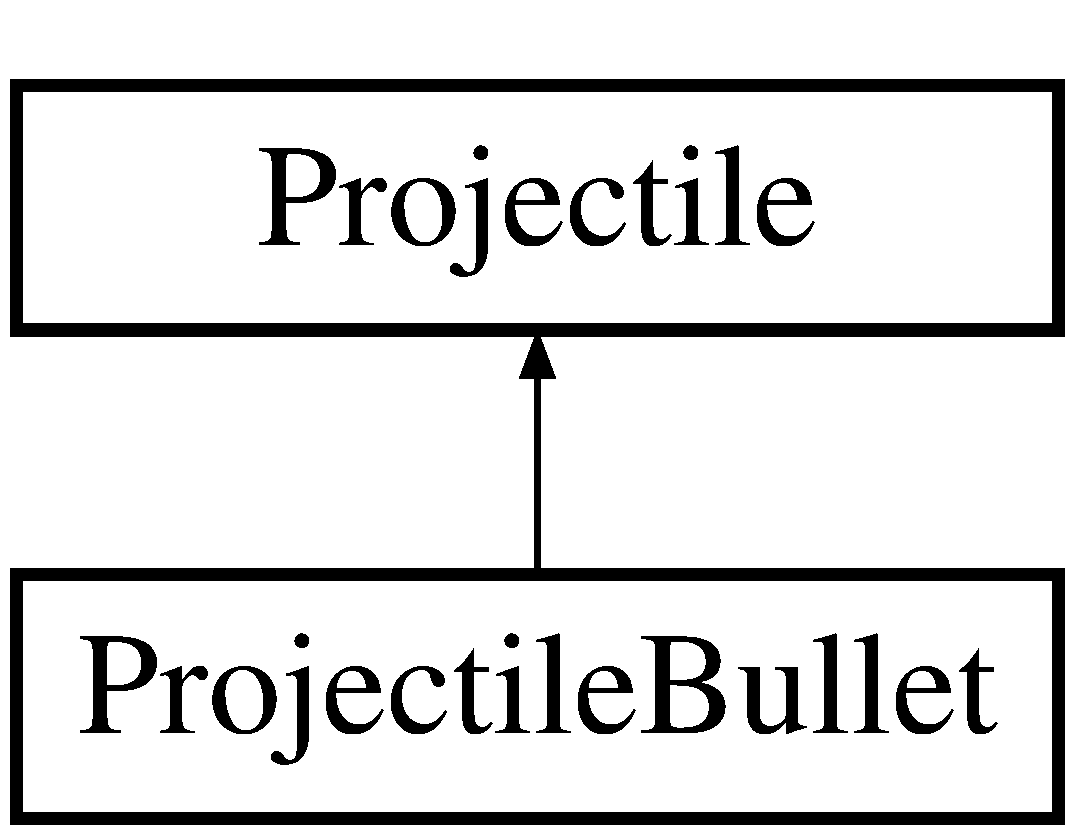
\includegraphics[height=2.000000cm]{class_projectile_bullet}
\end{center}
\end{figure}
\subsection*{Public Member Functions}
\begin{DoxyCompactItemize}
\item 
\hyperlink{class_projectile_bullet_a6d71699b04878b35c56b0268e5a27dae}{Projectile\+Bullet} (float x\+Posi, float y\+Posi, int dir, int dam)
\begin{DoxyCompactList}\small\item\em Constructor function. \end{DoxyCompactList}\item 
int \hyperlink{class_projectile_bullet_a4e9ac5190fa050732a28e9c620fff724}{Get\+Bullet\+Damage} ()
\begin{DoxyCompactList}\small\item\em Getter function for bullet\+Damage variable. \end{DoxyCompactList}\end{DoxyCompactItemize}
\subsection*{Additional Inherited Members}


\subsection{Constructor \& Destructor Documentation}
\index{Projectile\+Bullet@{Projectile\+Bullet}!Projectile\+Bullet@{Projectile\+Bullet}}
\index{Projectile\+Bullet@{Projectile\+Bullet}!Projectile\+Bullet@{Projectile\+Bullet}}
\subsubsection[{\texorpdfstring{Projectile\+Bullet(float x\+Posi, float y\+Posi, int dir, int dam)}{ProjectileBullet(float xPosi, float yPosi, int dir, int dam)}}]{\setlength{\rightskip}{0pt plus 5cm}Projectile\+Bullet\+::\+Projectile\+Bullet (
\begin{DoxyParamCaption}
\item[{float}]{x\+Posi, }
\item[{float}]{y\+Posi, }
\item[{int}]{dir, }
\item[{int}]{dam}
\end{DoxyParamCaption}
)}\hypertarget{class_projectile_bullet_a6d71699b04878b35c56b0268e5a27dae}{}\label{class_projectile_bullet_a6d71699b04878b35c56b0268e5a27dae}


Constructor function. 

Retrieval Methods Once again, to improve code reusability, an argument to specify the \hyperlink{class_projectile}{Projectile} hitbox size could and probably should be added, rather than using the magic number 5.

Constructors and Destructors


\begin{DoxyParams}{Parameters}
{\em x\+Posi} & Position on x axis to place new \hyperlink{class_projectile_bullet}{Projectile\+Bullet} at. \\
\hline
{\em y\+Posi} & Position on y axis to place new \hyperlink{class_projectile_bullet}{Projectile\+Bullet} at. \\
\hline
{\em dir} & Direction new projectile should travel, up or down. \\
\hline
{\em dam} & Damage the bullet should deal. \begin{DoxyVerb}        All ProjectileBullets have a hitbox size of 5, this is not specified
        in the constructor.
\end{DoxyVerb}
\\
\hline
\end{DoxyParams}
\begin{DoxyReturn}{Returns}
Initialized \hyperlink{class_projectile_bullet}{Projectile\+Bullet} object. 
\end{DoxyReturn}


\subsection{Member Function Documentation}
\index{Projectile\+Bullet@{Projectile\+Bullet}!Get\+Bullet\+Damage@{Get\+Bullet\+Damage}}
\index{Get\+Bullet\+Damage@{Get\+Bullet\+Damage}!Projectile\+Bullet@{Projectile\+Bullet}}
\subsubsection[{\texorpdfstring{Get\+Bullet\+Damage()}{GetBulletDamage()}}]{\setlength{\rightskip}{0pt plus 5cm}Projectile\+Bullet\+::\+Get\+Bullet\+Damage (
\begin{DoxyParamCaption}
{}
\end{DoxyParamCaption}
)}\hypertarget{class_projectile_bullet_a4e9ac5190fa050732a28e9c620fff724}{}\label{class_projectile_bullet_a4e9ac5190fa050732a28e9c620fff724}


Getter function for bullet\+Damage variable. 

Additional comments about \hyperlink{class_projectile_bullet_a4e9ac5190fa050732a28e9c620fff724}{Get\+Bullet\+Damage()} method (if any).

Retrieval Methods

\begin{DoxyReturn}{Returns}
Integer value. 
\end{DoxyReturn}


The documentation for this class was generated from the following files\+:\begin{DoxyCompactItemize}
\item 
\hyperlink{bullet_8h}{bullet.\+h}\item 
bullet.\+cpp\end{DoxyCompactItemize}

\chapter{File Documentation}
\hypertarget{actor_8cpp}{}\section{actor.\+cpp File Reference}
\label{actor_8cpp}\index{actor.\+cpp@{actor.\+cpp}}


Implementation of \hyperlink{class_actor}{Actor} class.  


{\ttfamily \#include $<$allegro5/allegro.\+h$>$}\\*
{\ttfamily \#include \char`\"{}actor.\+h\char`\"{}}\\*


\subsection{Detailed Description}
Implementation of \hyperlink{class_actor}{Actor} class. 

This contains the implementations of the public and private methods for the \hyperlink{class_actor}{Actor} class.

\begin{DoxyAuthor}{Author}
Tyler Bertram 
\end{DoxyAuthor}
\begin{DoxyRefDesc}{Bug}
\item[\hyperlink{bug__bug000001}{Bug}]No known bugs. \end{DoxyRefDesc}

\hypertarget{actor_8h}{}\section{actor.\+h File Reference}
\label{actor_8h}\index{actor.\+h@{actor.\+h}}


Definition of \hyperlink{class_actor}{Actor} class.  


{\ttfamily \#include $<$allegro5/allegro.\+h$>$}\\*
{\ttfamily \#include $<$string$>$}\\*
{\ttfamily \#include \char`\"{}Hitbox.\+h\char`\"{}}\\*
{\ttfamily \#include $<$memory$>$}\\*
\subsection*{Classes}
\begin{DoxyCompactItemize}
\item 
class \hyperlink{class_actor}{Actor}
\end{DoxyCompactItemize}


\subsection{Detailed Description}
Definition of \hyperlink{class_actor}{Actor} class. 

This contains the definitions of the public and private member variables, as well as all methods, for the \hyperlink{class_actor}{Actor} class, which handles basic functionality for any active \char`\"{}character\char`\"{} or similar in the game area (players, enemies, etc.).

\begin{DoxyAuthor}{Author}
Tyler Bertram 
\end{DoxyAuthor}
\begin{DoxyRefDesc}{Bug}
\item[\hyperlink{bug__bug000002}{Bug}]No known bugs. \end{DoxyRefDesc}

\hypertarget{actor_enemy_basic_8cpp}{}\section{actor\+Enemy\+Basic.\+cpp File Reference}
\label{actor_enemy_basic_8cpp}\index{actor\+Enemy\+Basic.\+cpp@{actor\+Enemy\+Basic.\+cpp}}


Implementation of \hyperlink{class_actor_enemy_basic}{Actor\+Enemy\+Basic} class.  


{\ttfamily \#include \char`\"{}actor\+Enemy\+Basic.\+h\char`\"{}}\\*


\subsection{Detailed Description}
Implementation of \hyperlink{class_actor_enemy_basic}{Actor\+Enemy\+Basic} class. 

This contains the implementations of all methods for the \hyperlink{class_actor_enemy_basic}{Actor\+Enemy\+Basic} class, which handles functionality specifically for the basic, or most average/typical enemy type in the game, notably also the only current enemy type in the game.

\begin{DoxyAuthor}{Author}
Tyler Bertram 
\end{DoxyAuthor}
\begin{DoxyRefDesc}{Bug}
\item[\hyperlink{bug__bug000003}{Bug}]If an enemy unit is spawned within 25 pixels of either screen edge, due to the move\+Actor logic, it will careen towards the bottom of the screen instead of correctly moving. Don\textquotesingle{}t place units within this space. \end{DoxyRefDesc}

\hypertarget{actor_enemy_basic_8h}{}\section{actor\+Enemy\+Basic.\+h File Reference}
\label{actor_enemy_basic_8h}\index{actor\+Enemy\+Basic.\+h@{actor\+Enemy\+Basic.\+h}}


Definition of \hyperlink{class_actor_enemy_basic}{Actor\+Enemy\+Basic} class.  


{\ttfamily \#include $<$allegro5/allegro.\+h$>$}\\*
{\ttfamily \#include \char`\"{}actor.\+h\char`\"{}}\\*
{\ttfamily \#include \char`\"{}Hitbox.\+h\char`\"{}}\\*
\subsection*{Classes}
\begin{DoxyCompactItemize}
\item 
class \hyperlink{class_actor_enemy_basic}{Actor\+Enemy\+Basic}
\end{DoxyCompactItemize}


\subsection{Detailed Description}
Definition of \hyperlink{class_actor_enemy_basic}{Actor\+Enemy\+Basic} class. 

This contains the definitions of the public and private member variables, as well as all methods, for the \hyperlink{class_actor_enemy_basic}{Actor\+Enemy\+Basic} class, which handles functionality specifically for the basic, or most average/typical enemy type in the game, notably also the only current enemy type in the game.

\begin{DoxyAuthor}{Author}
Tyler Bertram 
\end{DoxyAuthor}
\begin{DoxyRefDesc}{Bug}
\item[\hyperlink{bug__bug000004}{Bug}]If an enemy unit is spawned within 25 pixels of either screen edge, due to the move\+Actor logic, it will careen towards the bottom of the screen instead of correctly moving. Don\textquotesingle{}t place units within this space. \end{DoxyRefDesc}

\hypertarget{actor_player_8cpp}{}\section{actor\+Player.\+cpp File Reference}
\label{actor_player_8cpp}\index{actor\+Player.\+cpp@{actor\+Player.\+cpp}}


Implementation of \hyperlink{class_actor_player}{Actor\+Player} class.  


{\ttfamily \#include \char`\"{}actor\+Player.\+h\char`\"{}}\\*


\subsection{Detailed Description}
Implementation of \hyperlink{class_actor_player}{Actor\+Player} class. 

This contains the implementation of all methods for the \hyperlink{class_actor_player}{Actor\+Player} class, which handles all internal functionality for the player\textquotesingle{}s ship in the game.

\begin{DoxyAuthor}{Author}
Tyler Bertram 
\end{DoxyAuthor}
\begin{DoxyRefDesc}{Bug}
\item[\hyperlink{bug__bug000005}{Bug}]No known bugs. \end{DoxyRefDesc}

\hypertarget{actor_player_8h}{}\section{actor\+Player.\+h File Reference}
\label{actor_player_8h}\index{actor\+Player.\+h@{actor\+Player.\+h}}


Definition of \hyperlink{class_actor_player}{Actor\+Player} class.  


{\ttfamily \#include $<$allegro5/allegro.\+h$>$}\\*
{\ttfamily \#include \char`\"{}actor.\+h\char`\"{}}\\*
{\ttfamily \#include \char`\"{}Hitbox.\+h\char`\"{}}\\*
\subsection*{Classes}
\begin{DoxyCompactItemize}
\item 
class \hyperlink{class_actor_player}{Actor\+Player}
\end{DoxyCompactItemize}


\subsection{Detailed Description}
Definition of \hyperlink{class_actor_player}{Actor\+Player} class. 

This contains the definitions of the public and private member variables, as well as all methods, for the \hyperlink{class_actor_player}{Actor\+Player} class, which handles all internal functionality for the player\textquotesingle{}s ship in the game.

\begin{DoxyAuthor}{Author}
Tyler Bertram 
\end{DoxyAuthor}
\begin{DoxyRefDesc}{Bug}
\item[\hyperlink{bug__bug000006}{Bug}]No known bugs. \end{DoxyRefDesc}

\hypertarget{bullet_8h}{}\section{bullet.\+h File Reference}
\label{bullet_8h}\index{bullet.\+h@{bullet.\+h}}


Implementation of \hyperlink{class_projectile_bullet}{Projectile\+Bullet} class.  


{\ttfamily \#include \char`\"{}projectile.\+h\char`\"{}}\\*
{\ttfamily \#include $<$allegro5/allegro.\+h$>$}\\*
\subsection*{Classes}
\begin{DoxyCompactItemize}
\item 
class \hyperlink{class_projectile_bullet}{Projectile\+Bullet}
\end{DoxyCompactItemize}


\subsection{Detailed Description}
Implementation of \hyperlink{class_projectile_bullet}{Projectile\+Bullet} class. 

Definition of \hyperlink{class_projectile_bullet}{Projectile\+Bullet} class.

This contains the implementation of all methods for the \hyperlink{class_projectile_bullet}{Projectile\+Bullet} class, which is the primary vector of (violent) interaction between actors in the game space.

\begin{DoxyAuthor}{Author}
Tyler Bertram 
\end{DoxyAuthor}
\begin{DoxyRefDesc}{Bug}
\item[\hyperlink{bug__bug000007}{Bug}]No known bugs. \end{DoxyRefDesc}


This contains the definitions of the public and private member variables, as well as all methods, for the \hyperlink{class_projectile_bullet}{Projectile\+Bullet} class, which is the primary vector of (violent) interaction between actors in the game space.

\begin{DoxyAuthor}{Author}
Tyler Bertram 
\end{DoxyAuthor}
\begin{DoxyRefDesc}{Bug}
\item[\hyperlink{bug__bug000008}{Bug}]No known bugs. \end{DoxyRefDesc}

\hypertarget{_hitbox_8cpp}{}\section{Hitbox.\+cpp File Reference}
\label{_hitbox_8cpp}\index{Hitbox.\+cpp@{Hitbox.\+cpp}}


Implementation of \hyperlink{class_hitbox}{Hitbox} class.  


{\ttfamily \#include \char`\"{}Hitbox.\+h\char`\"{}}\\*


\subsection{Detailed Description}
Implementation of \hyperlink{class_hitbox}{Hitbox} class. 

This contains the implementation of all methods for the \hyperlink{class_hitbox}{Hitbox} class, which is the object responsible for detecting all collisions between objects within the gamespace.

\begin{DoxyAuthor}{Author}
Tyler Bertram 
\end{DoxyAuthor}
\begin{DoxyRefDesc}{Bug}
\item[\hyperlink{bug__bug000009}{Bug}]No known bugs. \end{DoxyRefDesc}

\hypertarget{_hitbox_8h}{}\section{Hitbox.\+h File Reference}
\label{_hitbox_8h}\index{Hitbox.\+h@{Hitbox.\+h}}


Definition of \hyperlink{class_hitbox}{Hitbox} class.  


{\ttfamily \#include $<$iostream$>$}\\*
\subsection*{Classes}
\begin{DoxyCompactItemize}
\item 
class \hyperlink{class_hitbox}{Hitbox}
\end{DoxyCompactItemize}


\subsection{Detailed Description}
Definition of \hyperlink{class_hitbox}{Hitbox} class. 

This contains the definitions of the public and private member variables, as well as all methods, for the \hyperlink{class_hitbox}{Hitbox} class, which is the object responsible for detecting all collisions between objects within the gamespace.

\begin{DoxyAuthor}{Author}
Tyler Bertram 
\end{DoxyAuthor}
\begin{DoxyRefDesc}{Bug}
\item[\hyperlink{bug__bug000010}{Bug}]No known bugs. \end{DoxyRefDesc}

\hypertarget{main_8cpp}{}\section{main.\+cpp File Reference}
\label{main_8cpp}\index{main.\+cpp@{main.\+cpp}}


An imitation of early S\+H\+M\+UP games like Galaga or Space Invaders. A C++ Allegro game for C\+P\+SC 2720 term project.  


{\ttfamily \#include $<$stdio.\+h$>$}\\*
{\ttfamily \#include $<$allegro5/allegro.\+h$>$}\\*
{\ttfamily \#include $<$allegro5/allegro\+\_\+native\+\_\+dialog.\+h$>$}\\*
{\ttfamily \#include $<$allegro5/allegro\+\_\+ttf.\+h$>$}\\*
{\ttfamily \#include $<$allegro5/allegro\+\_\+font.\+h$>$}\\*
{\ttfamily \#include $<$allegro5/allegro\+\_\+primitives.\+h$>$}\\*
{\ttfamily \#include $<$allegro5/allegro\+\_\+image.\+h$>$}\\*
{\ttfamily \#include $<$allegro5/allegro\+\_\+audio.\+h$>$}\\*
{\ttfamily \#include $<$allegro5/allegro\+\_\+acodec.\+h$>$}\\*
{\ttfamily \#include $<$iostream$>$}\\*
{\ttfamily \#include $<$vector$>$}\\*
{\ttfamily \#include $<$stdlib.\+h$>$}\\*
{\ttfamily \#include $<$time.\+h$>$}\\*
{\ttfamily \#include $<$map$>$}\\*
{\ttfamily \#include $<$algorithm$>$}\\*
{\ttfamily \#include \char`\"{}projectile.\+h\char`\"{}}\\*
{\ttfamily \#include \char`\"{}actor.\+h\char`\"{}}\\*
{\ttfamily \#include \char`\"{}bullet.\+h\char`\"{}}\\*
{\ttfamily \#include \char`\"{}actor\+Player.\+h\char`\"{}}\\*
{\ttfamily \#include \char`\"{}actor\+Enemy\+Basic.\+h\char`\"{}}\\*
{\ttfamily \#include \char`\"{}object\+Spawners.\+h\char`\"{}}\\*
\subsection*{Functions}
\begin{DoxyCompactItemize}
\item 
bool \hyperlink{main_8cpp_ad3cf59c57b6047ae36a44ae677fb1737}{enemy\+Remove\+Pred} (const \hyperlink{class_actor_enemy_basic}{Actor\+Enemy\+Basic} target)
\begin{DoxyCompactList}\small\item\em Predicate for remove\+\_\+if call on the basic enemy index. \end{DoxyCompactList}\item 
bool \hyperlink{main_8cpp_a2650a9e53ff5009b70ac4fbdba61716f}{bullet\+Remove\+Pred} (const \hyperlink{class_projectile_bullet}{Projectile\+Bullet} target)
\begin{DoxyCompactList}\small\item\em Predicate for remove\+\_\+if call on the bullet indices. \end{DoxyCompactList}\item 
int \hyperlink{main_8cpp_ae66f6b31b5ad750f1fe042a706a4e3d4}{main} ()
\end{DoxyCompactItemize}


\subsection{Detailed Description}
An imitation of early S\+H\+M\+UP games like Galaga or Space Invaders. A C++ Allegro game for C\+P\+SC 2720 term project. 

--Resource Credits-- Eric Skiff ( \href{http://ericskiff.com/music}{\tt http\+://ericskiff.\+com/music} ) for the music track Underclocked. Dalton Maag (\href{http://www.daltonmaag.com}{\tt http\+://www.\+daltonmaag.\+com} ) for the Ubuntu font.

\begin{DoxyAuthor}{Author}
Victor Adad, Tyler Bertram 
\end{DoxyAuthor}
\begin{DoxyRefDesc}{Bug}
\item[\hyperlink{bug__bug000011}{Bug}]No known bugs. \end{DoxyRefDesc}


\subsection{Function Documentation}
\index{main.\+cpp@{main.\+cpp}!bullet\+Remove\+Pred@{bullet\+Remove\+Pred}}
\index{bullet\+Remove\+Pred@{bullet\+Remove\+Pred}!main.\+cpp@{main.\+cpp}}
\subsubsection[{\texorpdfstring{bullet\+Remove\+Pred(const Projectile\+Bullet target)}{bulletRemovePred(const ProjectileBullet target)}}]{\setlength{\rightskip}{0pt plus 5cm}bullet\+Remove\+Pred (
\begin{DoxyParamCaption}
\item[{const {\bf Projectile\+Bullet}}]{target}
\end{DoxyParamCaption}
)}\hypertarget{main_8cpp_a2650a9e53ff5009b70ac4fbdba61716f}{}\label{main_8cpp_a2650a9e53ff5009b70ac4fbdba61716f}


Predicate for remove\+\_\+if call on the bullet indices. 


\begin{DoxyParams}{Parameters}
{\em target} & \hyperlink{class_projectile_bullet}{Projectile\+Bullet} type object. We check the proj\+Inactive boolian member and return its value.\\
\hline
\end{DoxyParams}
\begin{DoxyReturn}{Returns}
Boolian value. 
\end{DoxyReturn}
\index{main.\+cpp@{main.\+cpp}!enemy\+Remove\+Pred@{enemy\+Remove\+Pred}}
\index{enemy\+Remove\+Pred@{enemy\+Remove\+Pred}!main.\+cpp@{main.\+cpp}}
\subsubsection[{\texorpdfstring{enemy\+Remove\+Pred(const Actor\+Enemy\+Basic target)}{enemyRemovePred(const ActorEnemyBasic target)}}]{\setlength{\rightskip}{0pt plus 5cm}enemy\+Remove\+Pred (
\begin{DoxyParamCaption}
\item[{const {\bf Actor\+Enemy\+Basic}}]{target}
\end{DoxyParamCaption}
)}\hypertarget{main_8cpp_ad3cf59c57b6047ae36a44ae677fb1737}{}\label{main_8cpp_ad3cf59c57b6047ae36a44ae677fb1737}


Predicate for remove\+\_\+if call on the basic enemy index. 


\begin{DoxyParams}{Parameters}
{\em target} & \hyperlink{class_actor_enemy_basic}{Actor\+Enemy\+Basic} type object. We check the is\+Dead boolian member and return its value.\\
\hline
\end{DoxyParams}
\begin{DoxyReturn}{Returns}
Boolian value. 
\end{DoxyReturn}
\index{main.\+cpp@{main.\+cpp}!main@{main}}
\index{main@{main}!main.\+cpp@{main.\+cpp}}
\subsubsection[{\texorpdfstring{main()}{main()}}]{\setlength{\rightskip}{0pt plus 5cm}int main (
\begin{DoxyParamCaption}
{}
\end{DoxyParamCaption}
)}\hypertarget{main_8cpp_ae66f6b31b5ad750f1fe042a706a4e3d4}{}\label{main_8cpp_ae66f6b31b5ad750f1fe042a706a4e3d4}
$<$ Screen dimension constants.

$<$ Screen dimension constants.

$<$ Screen dimension constants.

$<$ Frames per second variable

$<$ If done == true, the game ends.

$<$ If draw == true, the gamestate will be drawn to the display.

$<$ Passed to the player object to control movement.

$<$ Passed to the player object to control movement.

$<$ If set to a negative value, the bullet will move in the opposite direction intended. This is undesirable behaviour.

$<$ If set to a negative value, the bullet will move in the opposite direction intended. This is undesirable behaviour.

$<$ Controls movement both of the player and enemies.

$<$ Random number storage variable for misc usage.

$<$ Random number storage variable for misc usage.

$<$ Used in animating the main menu/loading screen.

$<$ Vertical location in the menu bitmap to start drawing from.

$<$ Used to end the game when the player has completed all available stages. Note, the menu is considered stage 1, as the victory screen is stage 0 and death is stage -\/1.

$<$ If false, then displays main menu, if true, the \char`\"{}loading\char`\"{} screen will be shown.

$<$ Sums amount of time that the \char`\"{}loading\char`\"{} screen will be displayed.

$<$ Defines the current stage, which controls execution of certain code in the game loop. Initialized to 1 for the menu.

$<$ If true, the first-\/time enemy set-\/up for a stage will be performed. Initialized to true for this reason, so that the first stage sets up correctly.

$<$ Until allegro is initialized, this must be a null pointers.

Exception handling in the case that allegro does not initialize. This function M\+U\+ST be called first.

$<$ Sets up the previously declared display.

Exception handling in case the display fails to set up.

Initialize various allegro modules.

Initialization of Allegro-\/specific types that required the init funcs above in order to be declared.

$<$ A\+L\+L\+E\+G\+R\+O\+\_\+\+S\+A\+M\+P\+LE doesn\textquotesingle{}t support mp3 or midi files.

$<$ Indicate how many samples (sound files) we are using.

Syntax for sprite\+Index keys\+: x yz x\+: 0\+: abstract object, for instance buttons or menu elements; 1\+: actor sprites, for instance the player\textquotesingle{}s ship 2+\+: misc indices, unlikely to be used yz\+: order of loading. For instance, 000 is the first menu object loaded.

$<$ Plays the main theme.

Create the Player actor, and all required indices for game functions.

G\+A\+ME M\+A\+IN L\+O\+OP

$<$ After starting the timer, the only thing that should be done is the game loop, and subsequent object cleanup.

$<$ This is the game loop, right here.

$<$ waits for something to happen

$<$ I\+M\+P\+O\+R\+T\+A\+NT\+: gets the input from the keyboard

$<$ Updates and draws all elements in the game space.

$<$ Pressing escape key ends the program.

Game over screen, stage designate -\/1.

Victory screen, stage designate 0.

Menu screen, stage designate 1.

The following three conditional statements simply animate the menu screen, moving between two static images between update cycles.

Once the player presses enter, we begin the \char`\"{}loading\char`\"{} screen. Full disclosure\+: nothing is loading. However, the delay allows a player to prepare to play the game, rather than commencing play in the same second they press enter.

S\+T\+A\+GE S\+E\+T-\/\+UP

Stage Designate 2\+: Stage 1

Stage Designate 3\+: Stage 2

The stage is defeated when all basic enemies have been defeated, largely because the other non-\/boss enemy class we had wanted to implement would run off the screen and destruct itself automatically well before the player cleared out all of the basics.

P\+R\+E\+V\+I\+O\+US U\+P\+D\+A\+TE C\+L\+E\+A\+N\+UP

Any enemy which has moved off the bottom of the screen is no longer interesting/useful and can be safely deleted.

We only care if friendly bullets move off the top of the screen or hostile bullets move off the bottom. If friendly bullets are moving off the bottom or hostile bullets off the top, that\textquotesingle{}s incorrect behaviour.

U\+P\+D\+A\+TE P\+L\+A\+Y\+ER

Check if the player is dead, and also if the player has exhausted all their allotted lives.

$<$ Changes to the game over screen.

Get input and move the player accordingly.

Check if the player has flown into any of the enemy objects.

Control firing of friendly bullets.

U\+P\+D\+A\+TE E\+N\+E\+M\+I\+ES

Move all elements of each enemy index.

Check to see if any of the enemy objects have collided with the player.

Check to see if any enemy should fire a bullet, and if so, generate it.

One or no basic enemies will fire a bullet each update phase, depending on a certain percentile chance.

U\+P\+D\+A\+TE P\+R\+O\+J\+E\+C\+T\+I\+L\+ES

Move all bullets.

Check for collision between bullets and valid targets.

D\+R\+AW A\+LL O\+B\+J\+E\+C\+TS

Draw the player.

Draw the enemies.

Draw the bullets.

$<$ Updates the display.

$<$ Clear the display to the bg color in preparation for the next draw.

Clean up sprite\+Index.

Clean up unwrapped allegro objects.

End the program. 
\hypertarget{object_spawners_8cpp}{}\section{object\+Spawners.\+cpp File Reference}
\label{object_spawners_8cpp}\index{object\+Spawners.\+cpp@{object\+Spawners.\+cpp}}


Functions to create enemy and bullet objects for use in the game stages.  


{\ttfamily \#include \char`\"{}object\+Spawners.\+h\char`\"{}}\\*
\subsection*{Functions}
\begin{DoxyCompactItemize}
\item 
void \hyperlink{object_spawners_8cpp_a474db3fa38b1f3b0ad7726d922e6fcfd}{Spawn\+Bullet} (vector$<$ \hyperlink{class_projectile_bullet}{Projectile\+Bullet} $>$ \&target\+Index, float starting\+X\+Posi, float starting\+Y\+Posi, int damage, int direction)
\begin{DoxyCompactList}\small\item\em Constructor function. \end{DoxyCompactList}\item 
void \hyperlink{object_spawners_8cpp_af5cea0ac5d199480b9f685869b1e7cb7}{Spawn\+Basic\+Row} (vector$<$ \hyperlink{class_actor_enemy_basic}{Actor\+Enemy\+Basic} $>$ \&enemy\+Index, float starting\+X\+Posi, float starting\+Y\+Posi, int new\+Enemy\+Health, int new\+Enemy\+Score, int sprite\+Loc, bool right, int hitbox\+Size, int enemies\+To\+Spawn)
\end{DoxyCompactItemize}


\subsection{Detailed Description}
Functions to create enemy and bullet objects for use in the game stages. 

Implements the functions defined in \hyperlink{object_spawners_8h}{object\+Spawners.\+h}.

\begin{DoxyAuthor}{Author}
Tyler Bertram 
\end{DoxyAuthor}
\begin{DoxyRefDesc}{Bug}
\item[\hyperlink{bug__bug000012}{Bug}]No known bugs. \end{DoxyRefDesc}


\subsection{Function Documentation}
\index{object\+Spawners.\+cpp@{object\+Spawners.\+cpp}!Spawn\+Basic\+Row@{Spawn\+Basic\+Row}}
\index{Spawn\+Basic\+Row@{Spawn\+Basic\+Row}!object\+Spawners.\+cpp@{object\+Spawners.\+cpp}}
\subsubsection[{\texorpdfstring{Spawn\+Basic\+Row(vector$<$ Actor\+Enemy\+Basic $>$ \&enemy\+Index, float starting\+X\+Posi, float starting\+Y\+Posi, int new\+Enemy\+Health, int new\+Enemy\+Score, int sprite\+Loc, bool right, int hitbox\+Size, int enemies\+To\+Spawn)}{SpawnBasicRow(vector< ActorEnemyBasic > &enemyIndex, float startingXPosi, float startingYPosi, int newEnemyHealth, int newEnemyScore, int spriteLoc, bool right, int hitboxSize, int enemiesToSpawn)}}]{\setlength{\rightskip}{0pt plus 5cm}void Spawn\+Basic\+Row (
\begin{DoxyParamCaption}
\item[{vector$<$ {\bf Actor\+Enemy\+Basic} $>$ \&}]{enemy\+Index, }
\item[{float}]{starting\+X\+Posi, }
\item[{float}]{starting\+Y\+Posi, }
\item[{int}]{new\+Enemy\+Health, }
\item[{int}]{new\+Enemy\+Score, }
\item[{int}]{sprite\+Loc, }
\item[{bool}]{right, }
\item[{int}]{hitbox\+Size, }
\item[{int}]{enemies\+To\+Spawn}
\end{DoxyParamCaption}
)}\hypertarget{object_spawners_8cpp_af5cea0ac5d199480b9f685869b1e7cb7}{}\label{object_spawners_8cpp_af5cea0ac5d199480b9f685869b1e7cb7}
According to Dr. Memory (Windows memory leak detection tool), there may be a memory leak in this \index{object\+Spawners.\+cpp@{object\+Spawners.\+cpp}!Spawn\+Bullet@{Spawn\+Bullet}}
\index{Spawn\+Bullet@{Spawn\+Bullet}!object\+Spawners.\+cpp@{object\+Spawners.\+cpp}}
\subsubsection[{\texorpdfstring{Spawn\+Bullet(vector$<$ Projectile\+Bullet $>$ \&target\+Index, float starting\+X\+Posi, float starting\+Y\+Posi, int damage, int direction)}{SpawnBullet(vector< ProjectileBullet > &targetIndex, float startingXPosi, float startingYPosi, int damage, int direction)}}]{\setlength{\rightskip}{0pt plus 5cm}Spawn\+Bullet (
\begin{DoxyParamCaption}
\item[{vector$<$ {\bf Projectile\+Bullet} $>$ \&}]{target\+Index, }
\item[{float}]{starting\+X\+Posi, }
\item[{float}]{starting\+Y\+Posi, }
\item[{int}]{damage, }
\item[{int}]{direction}
\end{DoxyParamCaption}
)}\hypertarget{object_spawners_8cpp_a474db3fa38b1f3b0ad7726d922e6fcfd}{}\label{object_spawners_8cpp_a474db3fa38b1f3b0ad7726d922e6fcfd}


Constructor function. 

Implemented Functions Additional comments about Spawn\+Bullet function (if any).

Implemented Functions


\begin{DoxyParams}{Parameters}
{\em target\+Index} & Vector index to load the new bullet into. \\
\hline
{\em starting\+X\+Posi} & Initial x-\/axis position of the new bullet. \\
\hline
{\em starting\+Y\+Posi} & Initial y-\/axis position of the new bullet. \\
\hline
{\em damage} & Damage the new bullet should deal. \\
\hline
{\em direction} & Direction the new bullet should travel (0 = UP, 1 = D\+O\+WN, see directions\+\_\+c enum in \hyperlink{projectile_8h}{projectile.\+h}) \begin{DoxyVerb}        Loads a newly-constructed Bullet object into the specified vector index, where it can be acted upon
        as desired.\end{DoxyVerb}
\\
\hline
{\em enemy\+Index} & Vector index to load the basic enemies into. \\
\hline
{\em starting\+X\+Posi} & Initial x-\/axis position of the first enemy spawned. \\
\hline
{\em starting\+Y\+Posi} & Initial y-\/axis position of the row of enemies to be created. \\
\hline
{\em new\+Enemy\+Health} & Amount of health the new enemies should begin with. \\
\hline
{\em new\+Enemy\+Score} & Value of the new enemies when killed (not currently utilized). \\
\hline
{\em sprite\+Loc} & sprite\+Index key to draw the new enemies. \\
\hline
{\em right} & If true, the enemies will begin moving right. If false, they will begin moving left instead. \\
\hline
{\em hitbox\+Size} & Size of the hitbox of the spawned enemies. \\
\hline
{\em enemies\+To\+Spawn} & Number of enemies to spawn in the row. Each enemy will be spawned with a 10 pixel space between its sprite and the sprite of the previously spawned enemy, if any. \begin{DoxyVerb}        Creates a row of one or more enemies of ActorEnemyBasic type and inserts them into a target vector index.
        The row exists on only one y-axis location, but enemies are spawned rightwards of a defined starting location.\end{DoxyVerb}
 \\
\hline
\end{DoxyParams}

\hypertarget{object_spawners_8h}{}\section{object\+Spawners.\+h File Reference}
\label{object_spawners_8h}\index{object\+Spawners.\+h@{object\+Spawners.\+h}}


Functions to create enemy and bullet objects for use in the game stages.  


{\ttfamily \#include $<$vector$>$}\\*
{\ttfamily \#include $<$string$>$}\\*
{\ttfamily \#include \char`\"{}actor.\+h\char`\"{}}\\*
{\ttfamily \#include \char`\"{}actor\+Enemy\+Basic.\+h\char`\"{}}\\*
{\ttfamily \#include \char`\"{}projectile.\+h\char`\"{}}\\*
{\ttfamily \#include \char`\"{}bullet.\+h\char`\"{}}\\*
{\ttfamily \#include \char`\"{}Hitbox.\+h\char`\"{}}\\*
\subsection*{Functions}
\begin{DoxyCompactItemize}
\item 
void \hyperlink{object_spawners_8h_acb621607b3255e1c7cb70934504b09fb}{Spawn\+Bullet} (vector$<$ \hyperlink{class_projectile_bullet}{Projectile\+Bullet} $>$ \&target\+Index, float starting\+X\+Posi, float starting\+Y\+Posi, int damage, int direction)
\begin{DoxyCompactList}\small\item\em Constructor function. \end{DoxyCompactList}\item 
void \hyperlink{object_spawners_8h_af5cea0ac5d199480b9f685869b1e7cb7}{Spawn\+Basic\+Row} (vector$<$ \hyperlink{class_actor_enemy_basic}{Actor\+Enemy\+Basic} $>$ \&enemy\+Index, float starting\+X\+Posi, float starting\+Y\+Posi, int new\+Enemy\+Health, int new\+Enemy\+Score, int sprite\+Loc, bool right, int hitbox\+Size, int enemies\+To\+Spawn)
\end{DoxyCompactItemize}


\subsection{Detailed Description}
Functions to create enemy and bullet objects for use in the game stages. 

Each function defined below creates a certain number (either one or more) of a specific type of object which will activate and act as specified in the game space.

\begin{DoxyAuthor}{Author}
Tyler Bertram 
\end{DoxyAuthor}
\begin{DoxyRefDesc}{Bug}
\item[\hyperlink{bug__bug000013}{Bug}]No known bugs. \end{DoxyRefDesc}


\subsection{Function Documentation}
\index{object\+Spawners.\+h@{object\+Spawners.\+h}!Spawn\+Basic\+Row@{Spawn\+Basic\+Row}}
\index{Spawn\+Basic\+Row@{Spawn\+Basic\+Row}!object\+Spawners.\+h@{object\+Spawners.\+h}}
\subsubsection[{\texorpdfstring{Spawn\+Basic\+Row(vector$<$ Actor\+Enemy\+Basic $>$ \&enemy\+Index, float starting\+X\+Posi, float starting\+Y\+Posi, int new\+Enemy\+Health, int new\+Enemy\+Score, int sprite\+Loc, bool right, int hitbox\+Size, int enemies\+To\+Spawn)}{SpawnBasicRow(vector< ActorEnemyBasic > &enemyIndex, float startingXPosi, float startingYPosi, int newEnemyHealth, int newEnemyScore, int spriteLoc, bool right, int hitboxSize, int enemiesToSpawn)}}]{\setlength{\rightskip}{0pt plus 5cm}void Spawn\+Basic\+Row (
\begin{DoxyParamCaption}
\item[{vector$<$ {\bf Actor\+Enemy\+Basic} $>$ \&}]{enemy\+Index, }
\item[{float}]{starting\+X\+Posi, }
\item[{float}]{starting\+Y\+Posi, }
\item[{int}]{new\+Enemy\+Health, }
\item[{int}]{new\+Enemy\+Score, }
\item[{int}]{sprite\+Loc, }
\item[{bool}]{right, }
\item[{int}]{hitbox\+Size, }
\item[{int}]{enemies\+To\+Spawn}
\end{DoxyParamCaption}
)}\hypertarget{object_spawners_8h_af5cea0ac5d199480b9f685869b1e7cb7}{}\label{object_spawners_8h_af5cea0ac5d199480b9f685869b1e7cb7}
According to Dr. Memory (Windows memory leak detection tool), there may be a memory leak in this \index{object\+Spawners.\+h@{object\+Spawners.\+h}!Spawn\+Bullet@{Spawn\+Bullet}}
\index{Spawn\+Bullet@{Spawn\+Bullet}!object\+Spawners.\+h@{object\+Spawners.\+h}}
\subsubsection[{\texorpdfstring{Spawn\+Bullet(vector$<$ Projectile\+Bullet $>$ \&target\+Index, float starting\+X\+Posi, float starting\+Y\+Posi, int damage, int direction)}{SpawnBullet(vector< ProjectileBullet > &targetIndex, float startingXPosi, float startingYPosi, int damage, int direction)}}]{\setlength{\rightskip}{0pt plus 5cm}void Spawn\+Bullet (
\begin{DoxyParamCaption}
\item[{vector$<$ {\bf Projectile\+Bullet} $>$ \&}]{target\+Index, }
\item[{float}]{starting\+X\+Posi, }
\item[{float}]{starting\+Y\+Posi, }
\item[{int}]{damage, }
\item[{int}]{direction}
\end{DoxyParamCaption}
)}\hypertarget{object_spawners_8h_acb621607b3255e1c7cb70934504b09fb}{}\label{object_spawners_8h_acb621607b3255e1c7cb70934504b09fb}


Constructor function. 

Implemented Functions Additional comments about Spawn\+Bullet function (if any).

Implemented Functions


\begin{DoxyParams}{Parameters}
{\em target\+Index} & Vector index to load the new bullet into. \\
\hline
{\em starting\+X\+Posi} & Initial x-\/axis position of the new bullet. \\
\hline
{\em starting\+Y\+Posi} & Initial y-\/axis position of the new bullet. \\
\hline
{\em damage} & Damage the new bullet should deal. \\
\hline
{\em direction} & Direction the new bullet should travel (0 = UP, 1 = D\+O\+WN, see directions\+\_\+c enum in \hyperlink{projectile_8h}{projectile.\+h}) \begin{DoxyVerb}        Loads a newly-constructed Bullet object into the specified vector index, where it can be acted upon
        as desired.\end{DoxyVerb}
\\
\hline
{\em enemy\+Index} & Vector index to load the basic enemies into. \\
\hline
{\em starting\+X\+Posi} & Initial x-\/axis position of the first enemy spawned. \\
\hline
{\em starting\+Y\+Posi} & Initial y-\/axis position of the row of enemies to be created. \\
\hline
{\em new\+Enemy\+Health} & Amount of health the new enemies should begin with. \\
\hline
{\em new\+Enemy\+Score} & Value of the new enemies when killed (not currently utilized). \\
\hline
{\em sprite\+Loc} & sprite\+Index key to draw the new enemies. \\
\hline
{\em right} & If true, the enemies will begin moving right. If false, they will begin moving left instead. \\
\hline
{\em hitbox\+Size} & Size of the hitbox of the spawned enemies. \\
\hline
{\em enemies\+To\+Spawn} & Number of enemies to spawn in the row. Each enemy will be spawned with a 10 pixel space between its sprite and the sprite of the previously spawned enemy, if any. \begin{DoxyVerb}        Creates a row of one or more enemies of ActorEnemyBasic type and inserts them into a target vector index.
        The row exists on only one y-axis location, but enemies are spawned rightwards of a defined starting location.\end{DoxyVerb}
 \\
\hline
\end{DoxyParams}

\hypertarget{projectile_8cpp}{}\section{projectile.\+cpp File Reference}
\label{projectile_8cpp}\index{projectile.\+cpp@{projectile.\+cpp}}


Implementation of \hyperlink{class_projectile}{Projectile} class.  


{\ttfamily \#include \char`\"{}projectile.\+h\char`\"{}}\\*


\subsection{Detailed Description}
Implementation of \hyperlink{class_projectile}{Projectile} class. 

This contains the implementation for the methods of the \hyperlink{class_projectile}{Projectile} class, which handles the vectors of interaction between actors in the game.

\begin{DoxyAuthor}{Author}
Tyler Bertram 
\end{DoxyAuthor}
\begin{DoxyRefDesc}{Bug}
\item[\hyperlink{bug__bug000014}{Bug}]No known bugs. \end{DoxyRefDesc}

\hypertarget{projectile_8h}{}\section{projectile.\+h File Reference}
\label{projectile_8h}\index{projectile.\+h@{projectile.\+h}}


Definition of \hyperlink{class_projectile}{Projectile} class.  


{\ttfamily \#include $<$allegro5/allegro.\+h$>$}\\*
{\ttfamily \#include $<$allegro5/allegro\+\_\+primitives.\+h$>$}\\*
{\ttfamily \#include $<$string$>$}\\*
{\ttfamily \#include \char`\"{}Hitbox.\+h\char`\"{}}\\*
\subsection*{Classes}
\begin{DoxyCompactItemize}
\item 
class \hyperlink{class_projectile}{Projectile}
\end{DoxyCompactItemize}


\subsection{Detailed Description}
Definition of \hyperlink{class_projectile}{Projectile} class. 

This contains the definitions of the public and private member variables, as well as all methods, for the \hyperlink{class_projectile}{Projectile} class, which handles interactions between actors in the game.

\begin{DoxyAuthor}{Author}
Tyler Bertram 
\end{DoxyAuthor}
\begin{DoxyRefDesc}{Bug}
\item[\hyperlink{bug__bug000015}{Bug}]No known bugs. \end{DoxyRefDesc}

%--- End generated contents ---

% Index
\backmatter
\newpage
\phantomsection
\clearemptydoublepage
\addcontentsline{toc}{chapter}{Index}
\printindex

\end{document}
